%%%%%%%%%%%%%%%%%%%%%%%
% Binghampton Arithmetic Talk
%%%%%%%%%%%%%%%%%%%%%%%


{
%\setbeamercolor{background canvas}{bg=UniGray}
\begin{frame}
\titlepage
\end{frame}
}



% Mordell 
\begin{frame}
	\begin{thm}[Mordell, 1922]
	Let $E/\Q$ be an elliptic curve. Then the group of $\Q$-rational points on $E$, denoted $E(\Q)$, is a finitely generated abelian group. In particular,
		\[
		E(\Q) \cong \Z^{r_\Q} \oplus E(\Q)_\tors,
		\]
	where $r_\Q \geq 0$ is the rank of $E$ and $E(\Q)_\tors$ is the torsion subgroup.
	\end{thm}
	\begin{figure}[h]
	\centering
	\begin{subfigure}{0.3\textwidth}
	\captionsetup{labelformat=empty}
	\centering
	\fbox{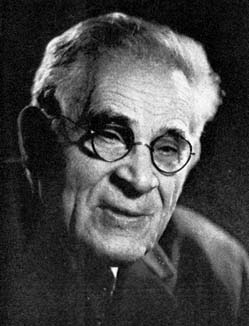
\includegraphics[width=0.8\textwidth]{images/mordell.jpg}}
	\caption{Louis J. Mordell}
	\end{subfigure}
	%
	\phantom{
	\begin{subfigure}{0.3\textwidth}
	\captionsetup{labelformat=empty}
	\centering
	\fbox{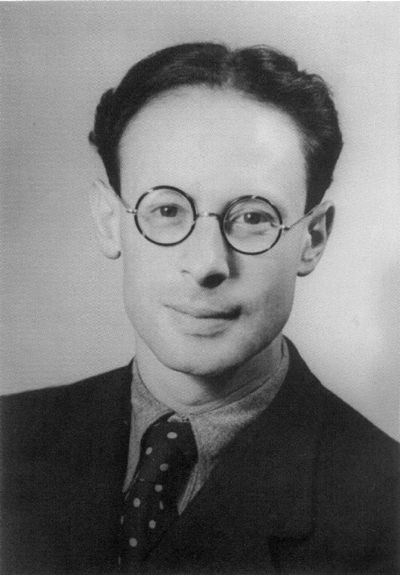
\includegraphics[width=0.74\textwidth]{images/weil.jpg}}
	\caption{Andr\'e Weil}
	\end{subfigure}
	%
	\begin{subfigure}{0.3\textwidth}
	\captionsetup{labelformat=empty}
	\centering
	\fbox{
\includegraphics[width=0.8\textwidth]{images/neron.png}}
	\caption{Andr\'e N\'eron}
	\end{subfigure}
	}
	\end{figure}
\end{frame}



% Mordell - Weil
\begin{frame}
	\begin{thm}[Mordell-Weil, 1928]
	Let $K$ be a number field, and let $A/K$ be an abelian variety. Then the group of $K$-rational points on $A$, denoted $A(K)$, is a finitely generated abelian group. In particular,
		\[
		A(K) \cong \Z^{r_K} \oplus A(K)_\tors,
		\]
	where $r_K \geq 0$ and $A(K)_\tors$ is the torsion subgroup.
	\end{thm}
	\begin{figure}[h]
	\centering
	\begin{subfigure}{0.3\textwidth}
	\captionsetup{labelformat=empty}
	\centering
	\fbox{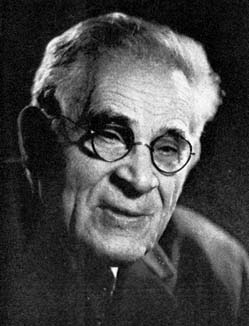
\includegraphics[width=0.8\textwidth]{images/mordell.jpg}}
	\caption{Louis J. Mordell}
	\end{subfigure}
	%
	\begin{subfigure}{0.3\textwidth}
	\captionsetup{labelformat=empty}
	\centering
	\fbox{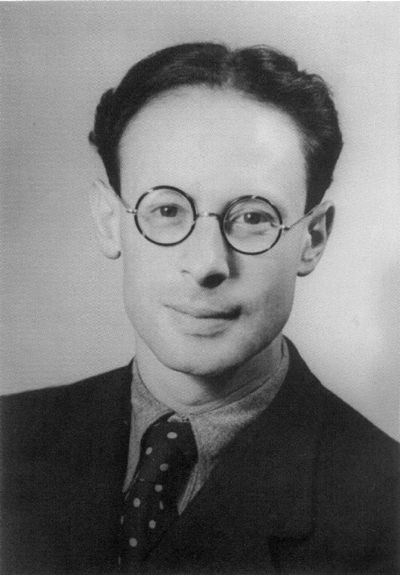
\includegraphics[width=0.74\textwidth]{images/weil.jpg}}
	\caption{Andr\'e Weil}
	\end{subfigure}
	%
	\phantom{
	\begin{subfigure}{0.3\textwidth}
	\captionsetup{labelformat=empty}
	\centering
	\fbox{
\includegraphics[width=0.8\textwidth]{images/neron.png}}
	\caption{Andr\'e N\'eron}
	\end{subfigure}
	}
	\end{figure}
\end{frame}



% Mordell - Weil - Neron
\begin{frame}
	\begin{thm}[Mordell-Weil-N\'eron, 1952]
	Let $K$ be a field that is finitely generated over its prime field, and let $A/K$ be an abelian variety. Then the group of $K$-rational points on $A$, denoted $A(K)$, is a finitely generated abelian group. In particular,
		\[
		A(K) \cong \Z^{r_K} \oplus A(K)_\tors,
		\]
	where $r_K \geq 0$ is the rank and $A(K)_\tors$ is the torsion subgroup. 
	\end{thm}
	\begin{figure}[h]
	\centering
	\begin{subfigure}{0.3\textwidth}
	\captionsetup{labelformat=empty}
	\centering
	\fbox{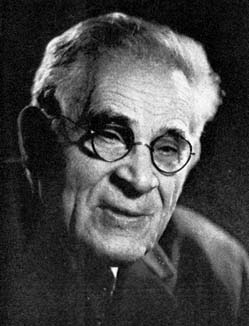
\includegraphics[width=0.8\textwidth]{images/mordell.jpg}}
	\caption{Louis J. Mordell}
	\end{subfigure}
	%
	\begin{subfigure}{0.3\textwidth}
	\captionsetup{labelformat=empty}
	\centering
	\fbox{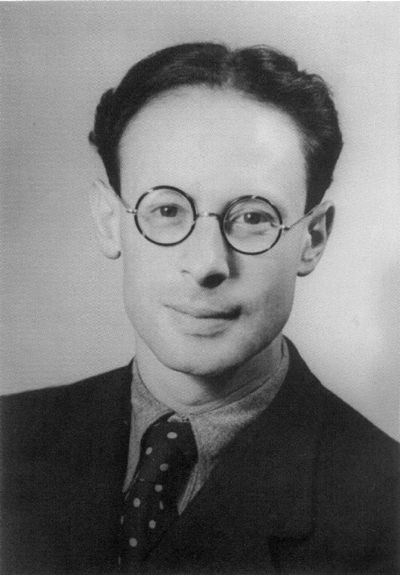
\includegraphics[width=0.74\textwidth]{images/weil.jpg}}
	\caption{Andr\'e Weil}
	\end{subfigure}
	%
	\begin{subfigure}{0.3\textwidth}
	\captionsetup{labelformat=empty}
	\centering
	\fbox{
\includegraphics[width=0.8\textwidth]{images/neron.png}}
	\caption{Andr\'e N\'eron}
	\end{subfigure}
	\end{figure}
\end{frame}



% Questions
\begin{frame}
\begin{ques}
What finitely generated abelian groups arise from abelian varieties over global fields?
\end{ques}
\end{frame}



% Questions
\begin{frame}
\ctext{This depends on what we vary.}
\end{frame}



% Questions
\begin{frame}
\begin{itemize}
\item Fix a global field $K$, and vary elliptic curves over $K$.
	\[
	E_1(K), \quad E_2(K), \quad \ldots \quad , \quad E_n(K), \quad \ldots
	\]  \pause

\item Fix an elliptic curve defined over $F$, and vary over finite extensions $K/F$
	\[
	\begin{tikzcd}[ampersand replacement=\&]
	E(K_1) \& E(K_2) \& \cdots \& E(K_n) \& \cdots \\
	\& \& E(F) \arrow[dash]{ull} \arrow[dash]{ul} \arrow[dash]{u} \arrow[dash]{ur} \arrow[dash]{urr} \& \& 
	\end{tikzcd}
	\]
where $K_1,K_2,\ldots,K_n,\ldots$ are in some family of finite extensions of $F$, contained in some fixed algebraic closure $\overline{F}$. Or vary over all elliptic curves over all extensions $\{K_n\}$. \pspace \pause

\item Take the previous question and replace $\{E_n(K)\}$ with an object of interest, e.g. $r_K, E_n(K)_\tors$, etc. 
\end{itemize}
\end{frame}



% What are Ranks?
\begin{frame}
\ctext{What are the possible ranks of elliptic curves $E/\Q$?}
\end{frame}



% Rank Records
\begin{frame}
	\begin{table}[h]
	\centering
	\begin{tabular}{lll}  
	{\itshape\large\bfseries Rank} & {\itshape\large\bfseries Year} & {\itshape\large\bfseries Due To} \\ \hline
	3 & 1938 & Billing \\ \rowcolor{UniOrange}
	\textcolor{white}{4} & \textcolor{white}{1945} &  \textcolor{white}{Wiman} \\ 
	6 & 1974 & Penney/Pomerance \\ \rowcolor{UniOrange}
	\textcolor{white}{7} & \textcolor{white}{1975} & \textcolor{white}{Penney/Pomerance} \\
	8 & 1977 & Grunewald/Zimmert \\ \rowcolor{UniOrange}
	\textcolor{white}{9} & \textcolor{white}{1977} & \textcolor{white}{Brumer/Kramer} \\
	12 & 1982 & Mestre \\ \rowcolor{UniOrange}
	\textcolor{white}{14} & \textcolor{white}{1986} & \textcolor{white}{Mestre} \\
	15 & 1992 &  Mestre \\  \rowcolor{UniOrange}
	\textcolor{white}{17} & \textcolor{white}{1992} & \textcolor{white}{Nagao} \\
	19 & 1992 & Fermigier \\ \rowcolor{UniOrange}
	\textcolor{white}{20} & \textcolor{white}{1993} & \textcolor{white}{Nagao} \\
	21 & 1994 & Nagao/Kouya \\ \rowcolor{UniOrange}
	\textcolor{white}{22} & \textcolor{white}{1997} & \textcolor{white}{Fermigier} \\
	23 & 1998 & Martin/McMillen \\ \rowcolor{UniOrange}
	\textcolor{white}{24} & \textcolor{white}{2000} & \textcolor{white}{Martin/McMillen} \\
	28 & 2006 & Elkies 
	\end{tabular}
	\end{table}
\end{frame}



% Time Series
\begin{frame}
%	\ctext{
%	\begin{figure}[!ht]
%	\centering
%	\includegraphics[width=0.80\textwidth]{images/ts.png}
%	\end{figure}
%	}
	\begin{figure}
	\centering
	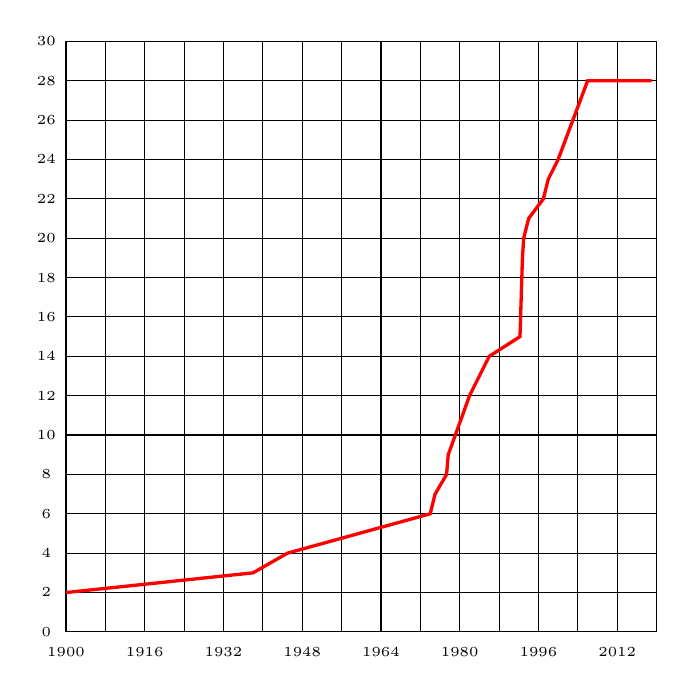
\begin{tikzpicture}[scale=0.50]%[scale=0.50, every node/.style={scale=0.1}]
	\foreach \k in {0,...,15}
		{
		\draw (\k,0) -- (\k,15);
		}
	\foreach \k in {0,...,15}
		{
		\draw (0,\k) -- (15,\k);
		}
	\node at (0,-0.5) {\tiny 1900};
	\node at (2,-0.5) {\tiny 1916};
	\node at (4,-0.5) {\tiny 1932};
	\node at (6,-0.5) {\tiny 1948};
	\node at (8,-0.5) {\tiny 1964};
	\node at (10,-0.5) {\tiny 1980};
	\node at (12,-0.5) {\tiny 1996};
	\node at (14,-0.5) {\tiny 2012};
	
	\node at (-0.5,0) {\tiny 0};
	\node at (-0.5,1) {\tiny 2};
	\node at (-0.5,2) {\tiny 4};
	\node at (-0.5,3) {\tiny 6};
	\node at (-0.5,4) {\tiny 8};
	\node at (-0.5,5) {\tiny 10};
	\node at (-0.5,6) {\tiny 12};
	\node at (-0.5,7) {\tiny 14};
	\node at (-0.5,8) {\tiny 16};
	\node at (-0.5,9) {\tiny 18};
	\node at (-0.5,10) {\tiny 20};
	\node at (-0.5,11) {\tiny 22};
	\node at (-0.5,12) {\tiny 24};
	\node at (-0.5,13) {\tiny 26};
	\node at (-0.5,14) {\tiny 28};
	\node at (-0.5,15) {\tiny 30};
	
	\draw[very thick,red] plot[samples=500] coordinates {
	(0,1)
	(4.75,1.5)
	(5.625,2)
	(9.25,3)
	(9.375,3.5)
	(9.6667,4)
	(9.7083,4.5)
	(10.25,6)
	(10.75,7)
	(11.5313,7.5)
	(11.5625,8.5)
	(11.5938,9.5)
	(11.625,10)
	(11.75,10.5)
	(12.125,11)
	(12.25,11.5)
	(12.5,12)
	(13.25,14)
	(14.875,14)
	};
	\end{tikzpicture}
	\end{figure}
\end{frame}



% Possible Ranks?
\begin{frame}
\ctext{Are the ranks of elliptic curves $E/\Q$ unbounded?}
\end{frame}



% BKLPR
\begin{frame}{\textcolor{white}{Some Heuristics}}

New heuristics of Jennifer Park, Bjorn Poonen, John Voight, and Melanie Matchett Wood model the distribution of Selmer groups, Tate-Shafarevich groups, and Mordell-Weil groups of `random' rational elliptic curves. \pause \par\vspace{0.3cm}

In particular, the $p$-adic Selmer group is modeled by the intersection between randomly chosen maximal isotropic subspaces in some large orthogonal spaces over $\Z_p$. \pause \par\vspace{0.3cm}

The model predicts\dots \pause
        \begin{itemize}
        \item $\text{rank } E(\Q)$ is 0 or 1 each with density 50\%. \pause
        \item $\text{rank } E(\Q) \geq 2$ with density 0\%. \pause
        \item Only finitely many elliptic curves over $\Q$ have rank $\geq 22$.
        \end{itemize}
\end{frame}



% What is Average Rank?
\begin{frame}
\ctext{What is the `average' rank of elliptic curves $E/\Q$?}
\end{frame}



% What is Average?
\begin{frame}
\ctext{What does `average' mean here?}
\end{frame}



% Infinite Set Probabilities
\begin{frame}[plain]
\noindent$\mathcal{A}:=$ Some property \par
\noindent$S_n:=$ set of objects up to size $n$. \par
\noindent$A_n:=$ set of objects in $S$ with property $\mathcal{A}$ in $S_n$. \vspace{1cm}
	\[
	\mu(\mathcal{A})= \lim_{n \to \infty} \dfrac{|A_n|}{|S_n|}
	\]
\end{frame}



% For Elliptic Curves
\begin{frame}
We need two things: \par\vspace{0.3cm}
	\begin{itemize}
	\item A notion of `size' for elliptic curves. \vspace{0.3cm}
	\item A way of counting the number of elliptic curves up to a given `size.'
	\end{itemize}
\end{frame}


% Elliptic Form
\begin{frame}
\textbf{Fact.} Any elliptic curve $E/\Q$ is isomorphic to an elliptic curve of the form
	\[
	E_{A,B} \colon y^2= x^3 + Ax + B.
	\] 
where $A,B \in \Z$. \pause \par\vspace{0.5cm}

In fact, $E/\Q$ is isomorphic to a unique $E_{A,B}$ if we require that if $p^4 \mid A$ then $p^6 \nmid B$. 
\end{frame}


% Size of Elliptic Curve
\begin{frame}
There are many notions of `size' (a.k.a. complexity) of an elliptic curve $E_{A,B}:= y^2= x^3+Ax+B$: \par\vspace{0.3cm}
	\begin{itemize}
	\item Na\"ive Height: $H(E_{A,B}):= \max\{|A|^3,|B|^2\}$ \fn{The na\"ive height can also be defined as $H(E_{A,B}):=\max\{4|A|^3,27B^2\}$.} \vfill
	\item Falting's Height \vfill
	\item Discriminant, $\Delta_E$: $\Delta(E_{A,B}):= -16(4A^3 + 27B^2)$ \vfill
	\item Conductor, $N_E:= \prod_{p \text{ prime}} p^{\,f_p(E)}$, where
		\[
		f_p(E)= \begin{cases}
		0, & E \text{ has good reduction at } p \\
		1, & E \text{ has multiplicative reduction at }p \\
		2, & E \text{ has additive reduction at }p
		\end{cases}
		\] \vfill
	\end{itemize}
\end{frame}



% Advantage
\begin{frame}
\frametitle{\textcolor{white}{Advantage of Na\"ive Height}}
Let $\mathcal{E}_{H \leq X}$ denote the set of isomorphism classes of elliptic curves of (na\"ive) height at most $X$. \pause 
	\[
	\#\mathcal{E}_{H \leq X} = 4 \zeta(10)^{-1} X^{5/6} + O(X^{1/2})
	\]  \pause
This essentially comes from the fact that there are $X^{1/3}$ choices for $A$ and $X^{1/2}$ choices for $B$. \pause \par\vspace{0.5cm}

It is conjectured that all the measures of heights give the same order of magnitude for all but a `small' proportion of elliptic curves. 
\end{frame}



% Goldfeld, Katz-Sarnak
\begin{frame}
	\begin{conj}[Goldfeld, Katz--Sarnak]
	When ordered by height, the average rank of elliptic curves $E/\Q$ is $\frac{1}{2}$. More precisely, 50\% of curves should have rank 0 and 50\% of curves should have rank 1.
	\end{conj}
	\begin{figure}[h]
	\centering
	\begin{subfigure}{0.3\textwidth}
	\captionsetup{labelformat=empty}
	\centering
	\fbox{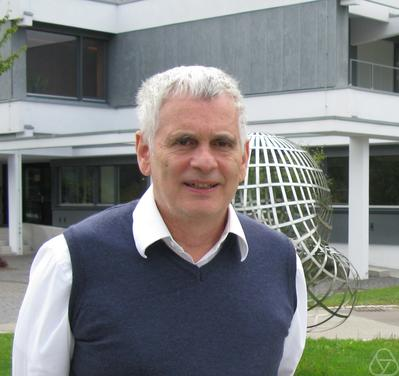
\includegraphics[width=\textwidth]{images/goldfeld.jpg}}
	\caption{\hspace{0.5cm}Dorian Goldfeld}
	\end{subfigure} \quad\quad
	%
	\begin{subfigure}{0.3\textwidth}
	\captionsetup{labelformat=empty}
	\centering
	\fbox{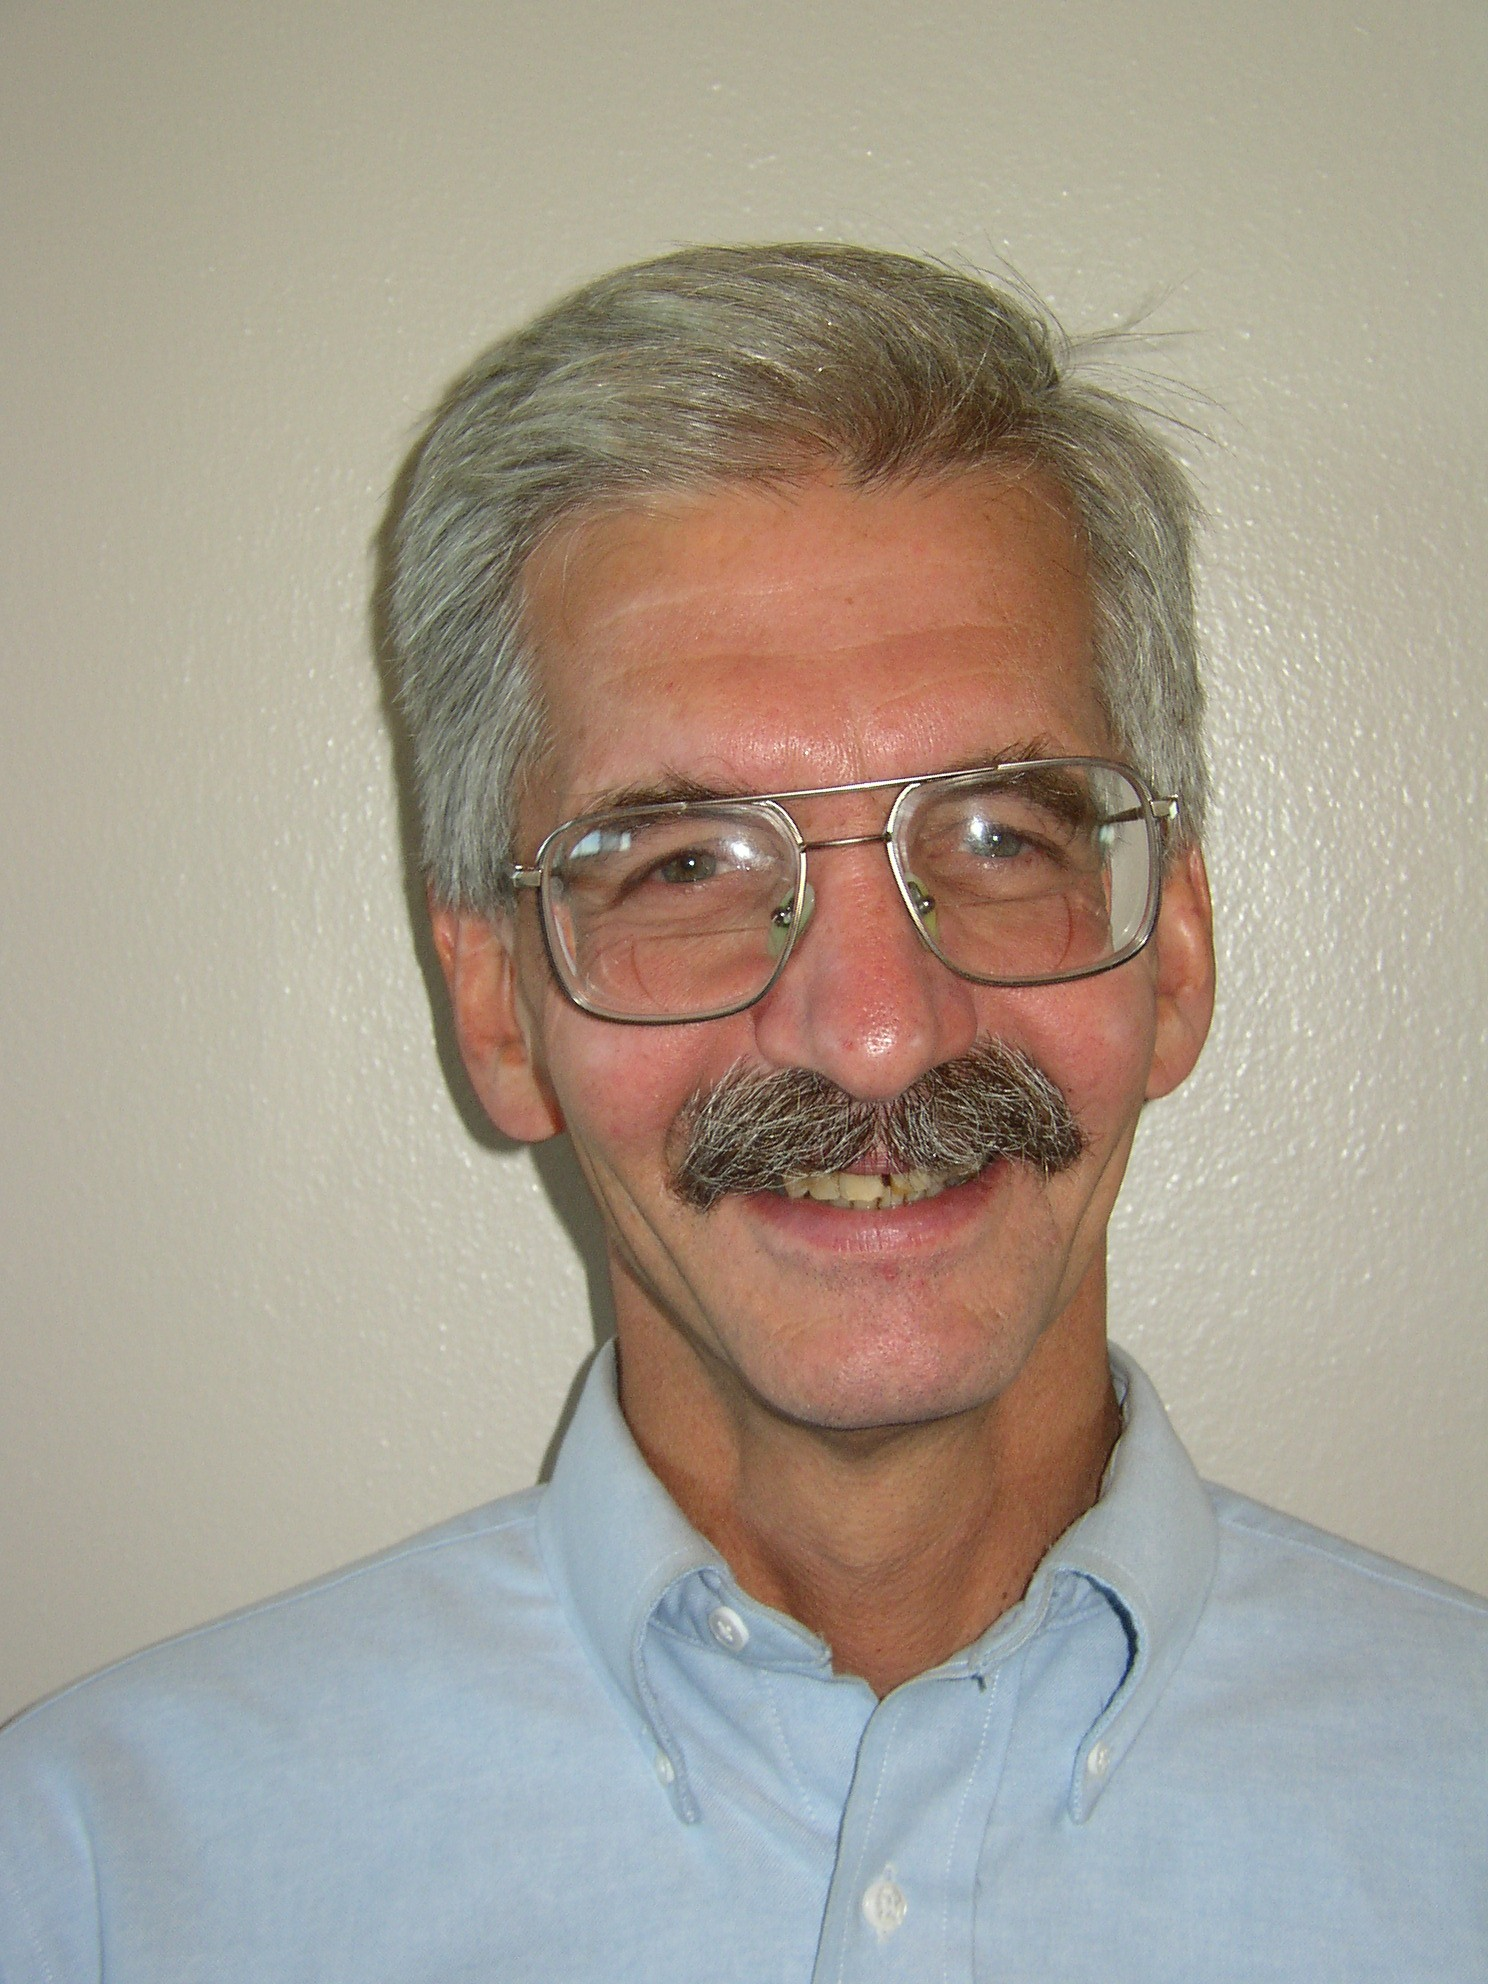
\includegraphics[width=0.72\textwidth]{images/katz.jpg}}
	\caption{Nick Katz}
	\end{subfigure}
	%
	\begin{subfigure}{0.3\textwidth}
	\captionsetup{labelformat=empty}
	\centering
	\fbox{
\includegraphics[width=0.65\textwidth]{images/sarnak.jpeg}}
	\caption{Peter Sarnak}
	\end{subfigure}
	\end{figure}
\end{frame}



% Previous
\begin{frame}
\ctext{Prior to the conjecture, the average rank was not even known to be finite!}
\end{frame}



% Graph 
\begin{frame}
\frametitle{\textcolor{white}{Computations of Brumer, McGuinness, Bektemirov, Stein, Watkins}}
	\begin{figure}
	\centering
	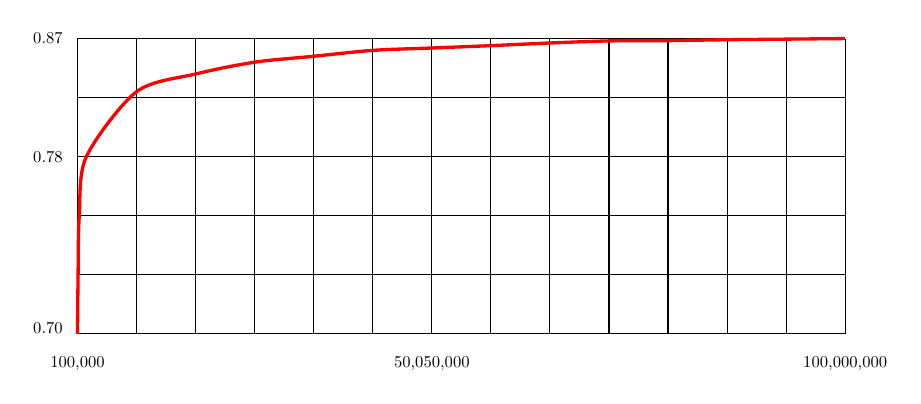
\begin{tikzpicture}[scale=0.75, every node/.style={scale=0.6}]
	\foreach \k in {0,...,13}
		{
		\draw (\k,0) -- (\k,5);
		}
	\foreach \k in {0,...,5}
		{
		\draw (0,\k) -- (13,\k);
		}
	\node at (0,-0.5) {100,000};
	\node at (6,-0.5) {50,050,000};
	\node at (13,-0.5) {100,000,000};
	
	\node at (-0.5,0.1) {0.70};
	\node at (-0.5,3) {0.78};
	\node at (-0.5,5) {0.87};
	\draw[very thick,red] plot[smooth] coordinates {
	(0,0) 
	(0.01,1) 
	(0.03,2) 
	(0.15,3)
	(1,4.1)
	(2,4.4)
	(3,4.6)
	(4,4.7)
	(5,4.8)
	(6,4.84)
	(7,4.88)
	(8,4.925)
	(9,4.96)
	(10,4.965)
	(11,4.98)
	(12,4.99)
	(13,5)
	};
	\end{tikzpicture}
	Average rank of elliptic curves of conductor $\leq 10^8$. The average turns out to be $0.8664\dots$. 
	\end{figure}
\end{frame}



% Previously Known
\begin{frame}
\frametitle{\textcolor{white}{Previously Known Results}}

\textbf{1992}: Assuming BSD \& GRH, Brumer showed the average rank is bounded (by 2.3). \pause \vfill

\textbf{2004}: Heath-Brown (assuming BSD, GRH) improved this average rank to $\leq 2.0$ \pause  \vfill

\textbf{2009}: Young (assuming BSD, GRH) improved this to $\leq 25/14 \approx 1.786$. \vfill
\end{frame}



% Unconditional
\begin{frame}[plain]
\ctext{Is there a proof of boundedness (with an estimate) without assuming BSD, GRH?}
\end{frame}



% Bhargava-Shankar
\begin{frame}[plain]
	\begin{figure}[h]
	\centering
	\begin{subfigure}{0.4\textwidth}
	\captionsetup{labelformat=empty}
	\centering
	\fbox{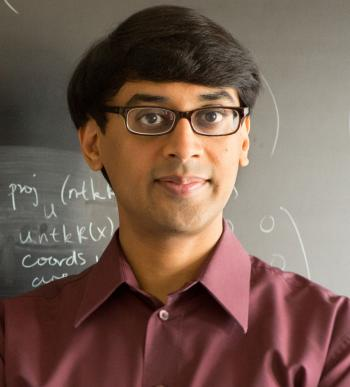
\includegraphics[width=0.7\textwidth]{images/bhargava.jpg}}
	\caption{Manjul Bhargava}
	\end{subfigure}
	%
	\begin{subfigure}{0.4\textwidth}
	\captionsetup{labelformat=empty}
	\centering
	\fbox{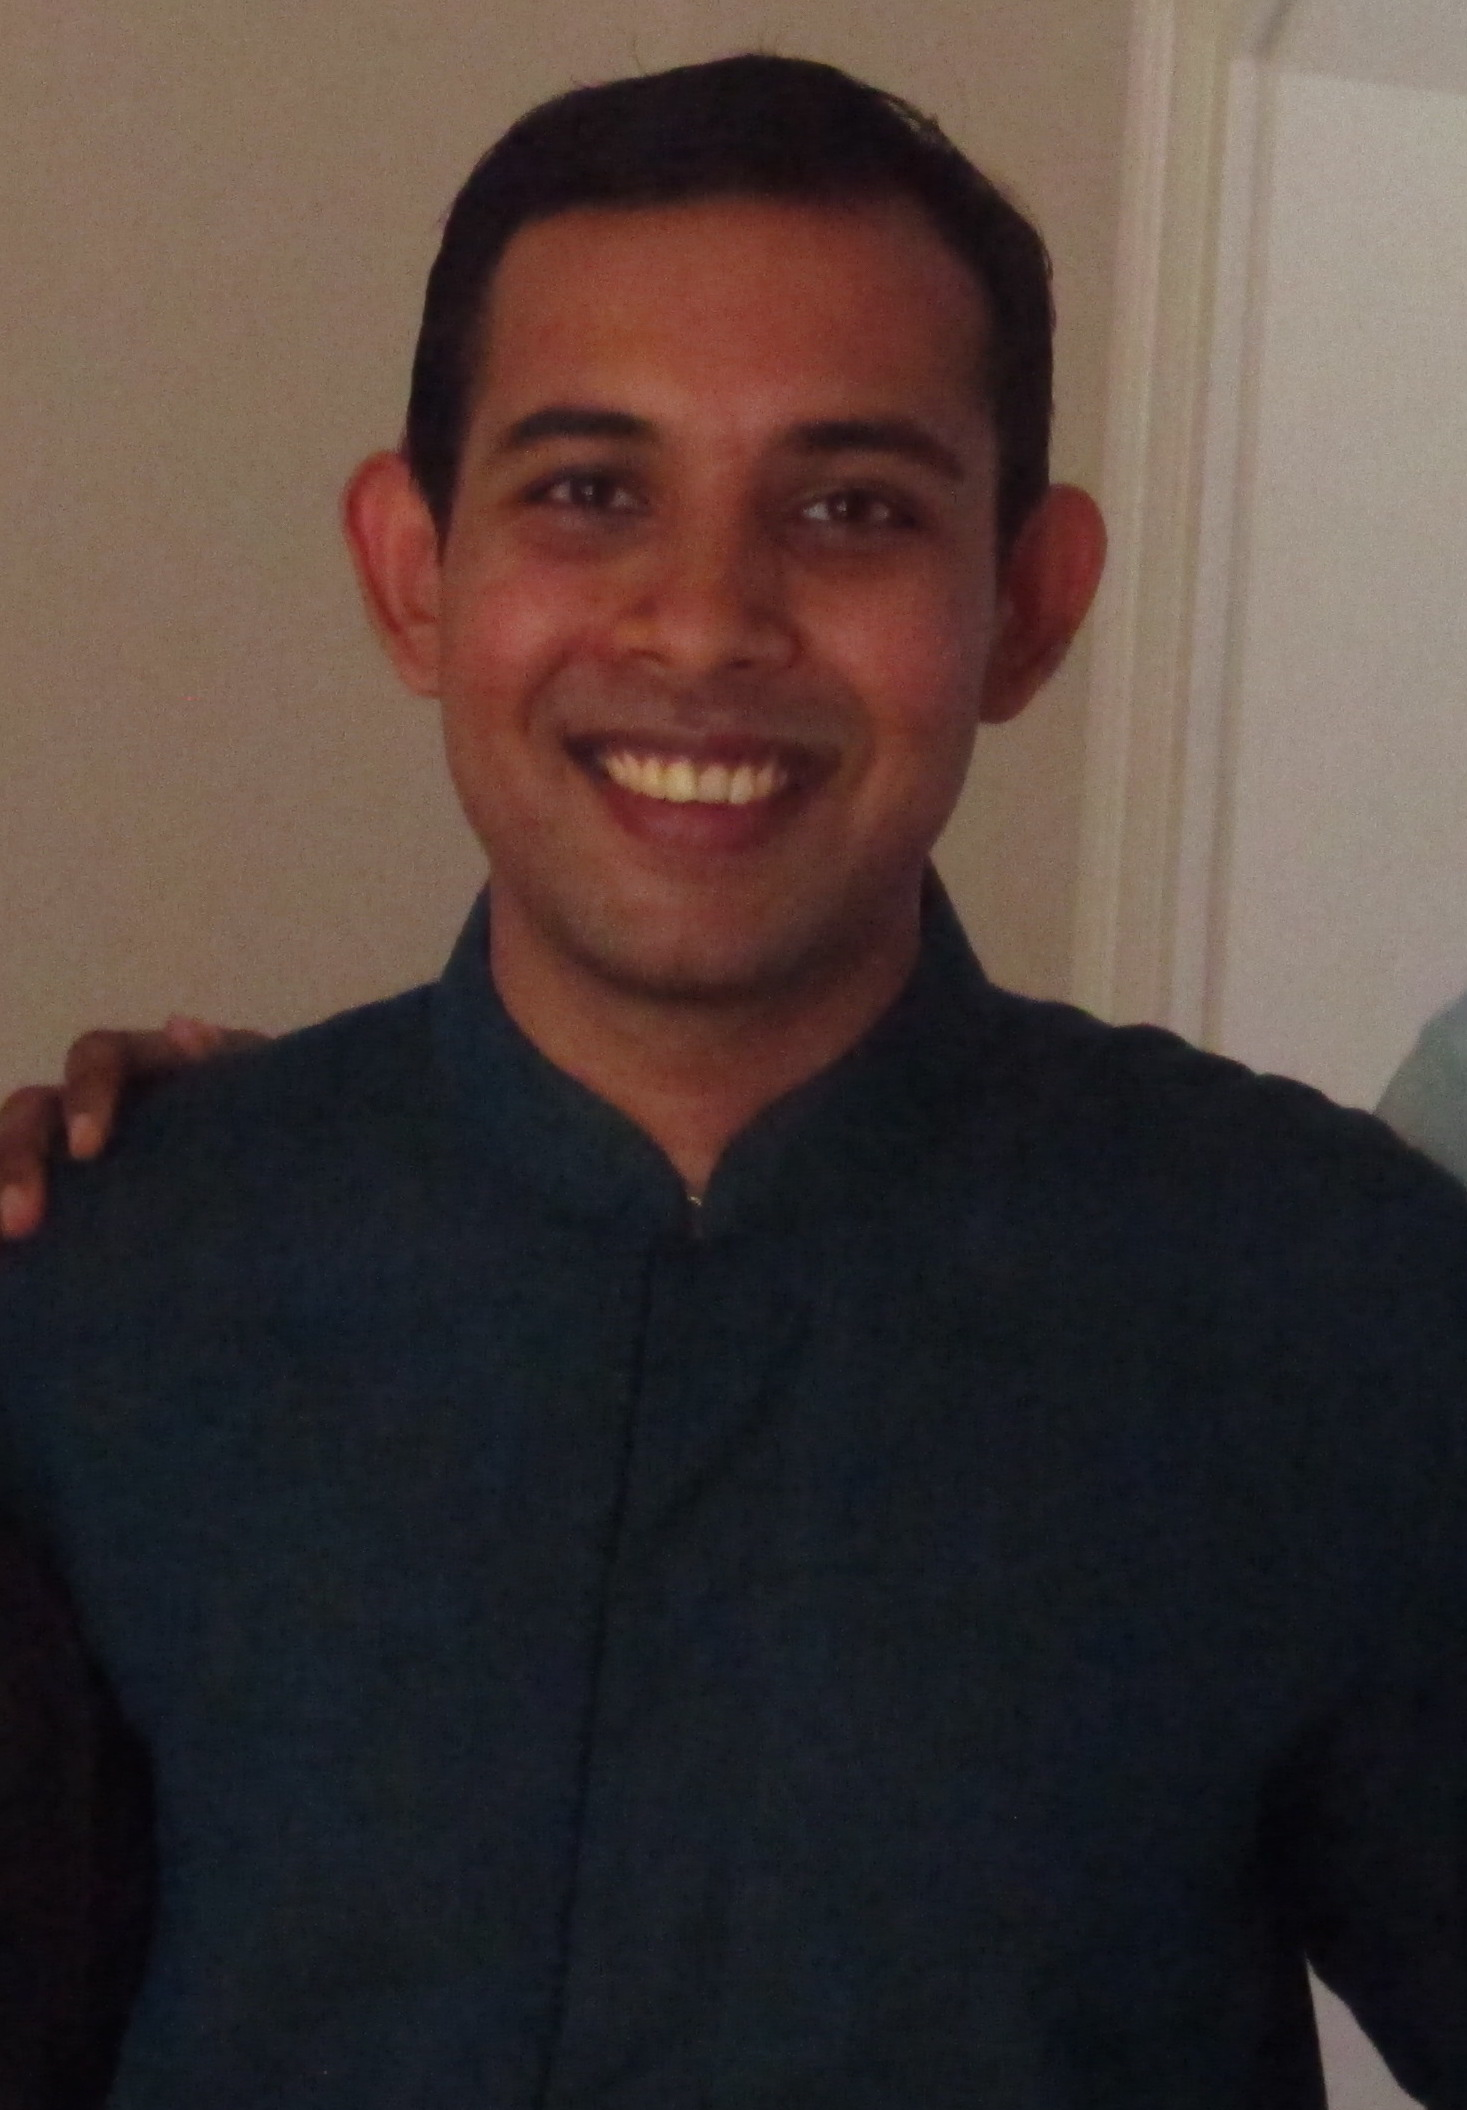
\includegraphics[width=0.55\textwidth]{images/shankar.jpg}}
	\caption{Arul Shankar}
	\end{subfigure}
	\end{figure}
\end{frame}



% Selmer \& Sha Intro
\begin{frame}
\frametitle{\textcolor{white}{Idea of Bhargava-Shankar}}

We do not know how to compute $E(\Q)$, so we study the `simpler' group $E(\Q)/nE(\Q)$. \pause \par \vspace{0.75cm}

By the Mordell-Weil Theorem, we know that 

	\[
	E(\Q) \cong \Z^r \oplus E(\Q)_\tors
	\] \pause 

Then we must have
	\[
	E(\Q)/nE(\Q) \cong (\Z/n\Z)^r \oplus E(\Q)_\tors/nE(\Q)_\tors
	\]
\end{frame}



% Selmer \& Sha Intro Cont
\begin{frame}
\frametitle{\textcolor{white}{Idea of Bhargava-Shankar}}
If we knew $E(\Q)/nE(\Q)$ and $E(\Q)_\tors$, we could compute $r$. \pause \par \vspace{0.5cm}

\textbf{Example.} If $n=p$, then
	\[
	\dim_{\F_p} E(\Q)/pE(\Q)= \dim_{\F_p} E(\Q)[p] + \rank E(\Q)
	\]
\end{frame}



% Selmer \& Sha
\begin{frame}
\frametitle{\textcolor{white}{Selmer \& Shafarevich-Tate Groups}}
Define a computable group $S^n(E)$, called the Selmer group, containing $E(\Q)/nE(\Q)$. \pause \par \vspace{0.5cm}

Approximate $E(\Q)/nE(\Q)$ by $S^{(n)}(E)$. We define an `error term' $\sha(E)$, called the Shafarevich-Tate group. 
	\[
	0 \ma{} E(\Q)/nE(\Q) \ma{} S^{(n)}(E) \ma{} \sha[n] \ma{} 0
	\]
\end{frame}



% Selmer \& Sha
\begin{frame}
\begin{dfn}
Let $\varphi: E/K \to E'/K$ be an isogeny. The $\varphi$-Selmer group $E/K$ is the subgroup of $H^1(G_{\overline{K}/K}, E[\varphi])$ defined by
	\[
	S^{(\varphi)}(E/K):= \ker \left\{ H^1(G_{\overline{K}/K}, E[\varphi]) \ma{} \prod_{v \in M_K} \text{WC}(E/K_v) \right\}
	\]
The Shafarevich-Tate group of $E/K$ is the subgroup of $\text{WC}(E/K)$ defined by
	\[
	\sha(E/K):= \ker \left\{ \text{WC}(E/K) \ma{} \prod_{v \in M_K} \text{WC}(E/K_v) \right\}.
	\]
\end{dfn}
\end{frame}



% Idea
\begin{frame}
\frametitle{\textcolor{white}{Idea of Bhargava-Shankar}}
	\[
	0 \ma{} E(\Q)/nE(\Q) \ma{} S^{(n)}(E) \ma{} \sha[n] \ma{} 0
	\] \vfill
	
If $E(\Q)[n]= \{\mathcal{O}\}$, then
	\[
	n^{\rank E} \leq |S^{(n)}(E)|.
	\] \pause \vspace{0.3cm}

To prove boundedness of average rank, it is enough to show that the average size of $|S^{(n)}(E)|$ for any $n>1$. 
\end{frame}



% Proof Outline
\begin{frame}
\frametitle{\textcolor{white}{Outline of the Proof}}
\begin{enumerate}[1.]
\item For $n \leq 5$, construct a representation $V$ of an algebraic group $G$ defined over $\Z$ related to $A,B$.
\item Count the elements under the action of $G$ on $V$ with bounded $A,B$.
\item Sieve to count the elements of $S^{(n)}(E_{A,B})$ `in' the representation.
\end{enumerate}
\end{frame}



% Bhargava - Shankar 
\begin{frame}
\begin{thm}[Bhargava--Shankar]
Let $n=1,2,3,4,5$. When elliptic curves $E/\Q$ are ordered by height, the average number of order $n$ elements in the $n$-Selmer group is $n$.
\end{thm} \pause

\begin{cor}
Let $n= 1,2,3,4,5$. When ordered by height, the average size of the $n$-Selmer group for elliptic curves $E/\Q$ is $\sigma(n)$.
\end{cor} \pause

\begin{conj}[Bhargava--Shankar]
Let $n \geq 1$. When elliptic curves $E/\Q$ are ordered by height, the average size of the $n$-Selmer group is $\sigma(n)$.
\end{conj}
\end{frame}



% Relation to Avg Rank
\begin{frame}
\begin{prop}[Bhargava--Shankar]
If the previous conjecture is true for all $n$, then when elliptic curves are ordered by height, a density of 100\% of elliptic curves have rank 0 or 1. 
\end{prop}
\end{frame}



% Avg Rank
\begin{frame}
\begin{thm}[Bhargava--Shankar]
When elliptic curves $E/\Q$ are ordered by height, the average rank is bounded (by $0.885<1$). 
\end{thm} \pause

\begin{cor}
When elliptic curves $E/\Q$ are ordered by height, a positive proportion have rank 0.
\end{cor}

\begin{cor}
When elliptic curves $E/\Q$ are ordered by height, more than 80\% have rank 0 or 1. 
\end{cor}
\end{frame}



% Rank 1
\begin{frame}[plain]
\begin{thm}[Bhargava, Shankar, Skinner]
When elliptic curves $E/\Q$ are ordered by height, a positive proportion have rank 1. 
\end{thm}
\end{frame}



% Analytic Rank
\begin{frame}
\begin{thm}[Bhargava--Shankar]
When elliptic curves $E/\Q$ are ordered by height, a positive proportion have analytic rank 0.
\end{thm} \pause

\begin{thm}[Bhargava--Shankar]
When elliptic curves $E/\Q$ are ordered by height, a positive proportion have analytic rank 1.
\end{thm} \pause

\begin{cor}
A positive proportion of elliptic curves satisfy the BSD conjecture. 
\end{cor} \pause

\begin{thm}[Bhargava--Shankar--Zhang]
More than 66\% of elliptic curves have analytic rank 0 or 1, and thus satisfy BSD.
\end{thm}
\end{frame}



% What about Torsion?
\begin{frame}
\ctext{What about Torsion?}
\end{frame}



% Q-Torsion (Mazur)
\begin{frame}[plain]
\begin{thm}[Levi-Ogg Conjecture; Mazur, 1977]
If $E/\Q$ is a rational elliptic curve, then the possible torsion subgroups $E(\Q)_\tors$ are precisely:
	\[
	\begin{cases}
	\Z/n\Z, & n=1,2,\ldots,10,12 \\
	\Z/2\Z \oplus \Z/2n\Z, & n=1,\ldots,4
	\end{cases}
	\]
Furthermore, each possibility occurs infinitely often.
\end{thm}
	\begin{figure}[h]
	\centering
	\begin{subfigure}{0.3\textwidth}
	\captionsetup{labelformat=empty}
	\centering
	\fbox{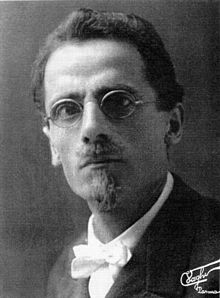
\includegraphics[width=0.72\textwidth]{images/levi.jpg}}
	\caption{Beppo Levi}
	\end{subfigure}
	%
	\begin{subfigure}{0.3\textwidth}
	\captionsetup{labelformat=empty}
	\centering
	\fbox{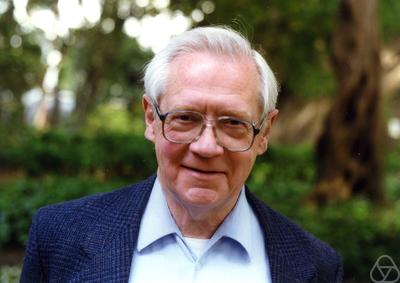
\includegraphics[width=\textwidth]{images/ogg.jpg}}
	\caption{Andrew Ogg}
	\end{subfigure} \hspace{0.05cm}
	%
	\begin{subfigure}{0.3\textwidth}
	\captionsetup{labelformat=empty}
	\centering
	\fbox{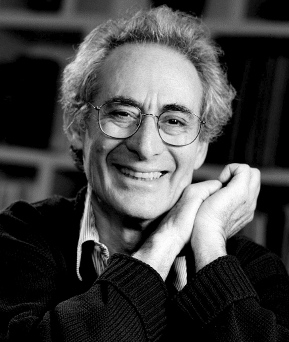
\includegraphics[width=0.82\textwidth]{images/mazur.jpg}}
	\caption{Barry Mazur}
	\end{subfigure}
	\end{figure}
\end{frame}



% Number Fields
\begin{frame}
\ctext{What about the groups $E(K)_\tors$, where $K$ is a number field of degree $d$?}
\end{frame}



% Joke
\begin{frame}
\ctext{With massive loss of generality, let $d=2$}
\end{frame}



% Quadratic
\begin{frame}[plain]
\begin{thm}[Kenku, Momose, 1988; Kamienny, 1992]
 Let $K/\Q$ be a quadratic number field and $E/K$ be an elliptic curve. Then the possible torsion subgroups $E(K)_\tors$ are precisely:
 	\[
	\begin{cases}
	\Z/n\Z, & n=1,2,\ldots,16,18 \\
	\Z/2\Z \oplus \Z/2n\Z, & n=1,\ldots,6 \\
	\Z/3\Z \oplus \Z/3n\Z, & n=1,2 \\
	\Z/4\Z \oplus \Z/4\Z
	\end{cases}
	\]
Moreover, each possibility occurs infinitely often. 
\end{thm}
	\begin{figure}[h]
	\centering
	\begin{subfigure}{0.3\textwidth}
	\captionsetup{labelformat=empty}
	\centering
	\fbox{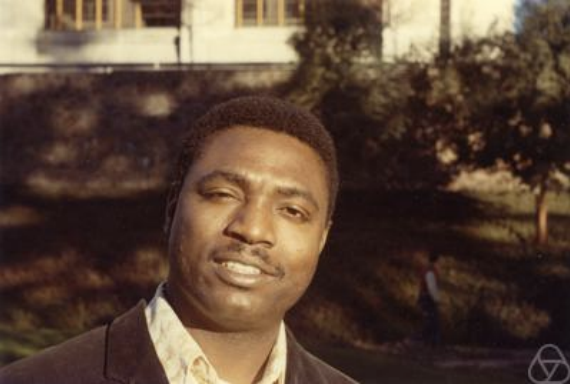
\includegraphics[width=0.9\textwidth]{images/kenku.png}}
	\caption{Monsur Kenku}
	\end{subfigure} \;\;\;
	%
	\begin{subfigure}{0.3\textwidth}
	\captionsetup{labelformat=empty}
	\centering
	\fbox{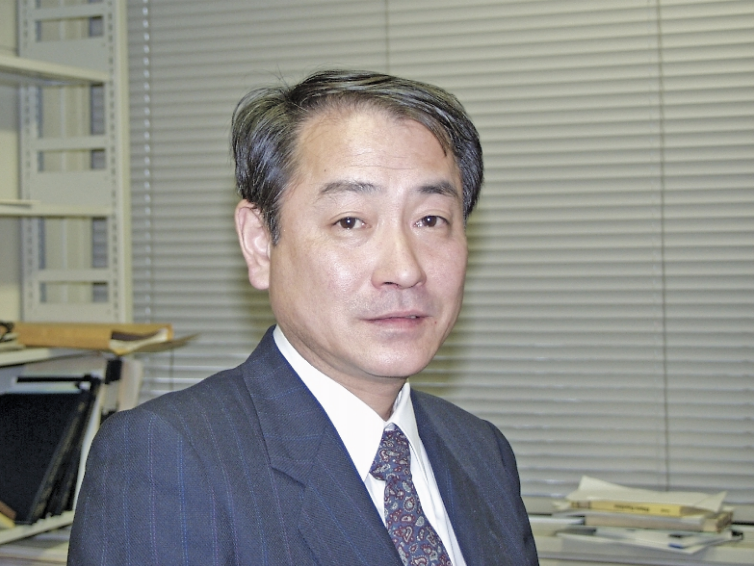
\includegraphics[width=0.85\textwidth]{images/momose.png}}
	\caption{Fumiyuki Momose}
	\end{subfigure}
	%
	\begin{subfigure}{0.3\textwidth}
	\captionsetup{labelformat=empty}
	\centering
	\fbox{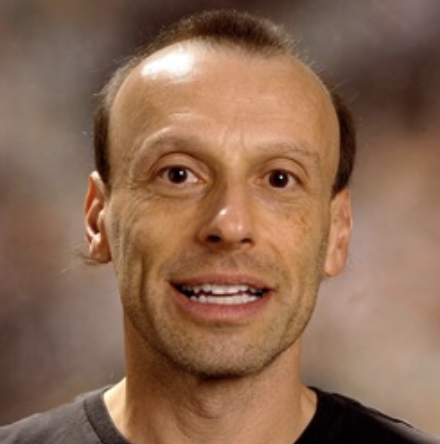
\includegraphics[width=0.63\textwidth]{images/kamienny.png}}
	\caption{Sheldon Kamienny}
	\end{subfigure}
	\end{figure}
\end{frame}



% Cubic
\begin{frame}[plain]
\begin{thm}[Jeon,Kim,Schweizer, 2004; Etropolski-Morrow-Zureick Brown; Derickx, 2016]
Let $K/\Q$ be a cubic number field and $E/K$ be an elliptic curve. Then the possible torsion subgroups $E(K)_\tors$ are precisely:
	\[
	\begin{cases}
	\Z/n\Z, & n=1,2,\ldots,16,18,20,21 \\
	\Z/2n\Z, & n=1,\ldots,7
	\end{cases}
	\] 
Each of these possibilities occurs infinitely many times except $\Z/21\Z$.
\end{thm}
	\begin{figure}[h]
	\centering
	\begin{subfigure}{0.10\textwidth}
	\captionsetup{labelformat=empty}
	\centering
	\fbox{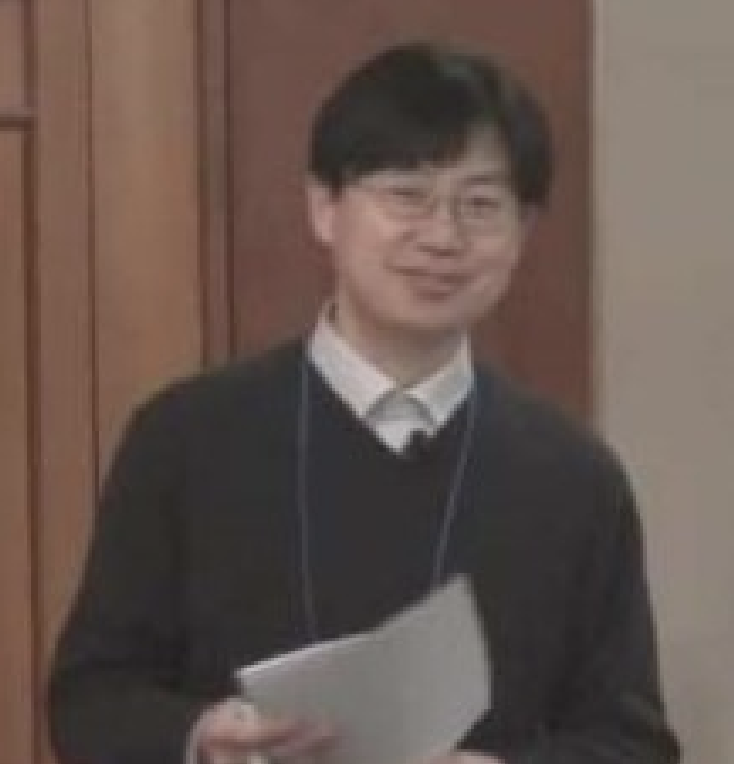
\includegraphics[width=1.2\textwidth]{images/jeon.png}}
	\caption{\hspace{0.2cm}\scriptsize{Jeon}}
	\end{subfigure} \quad\quad
	%
	\begin{subfigure}{0.10\textwidth}
	\captionsetup{labelformat=empty}
	\centering
	\fbox{
\includegraphics[width=1.2\textwidth]{images/kim.jpg}}
	\caption{\hspace{0.3cm}\scriptsize{Kim}}
	\end{subfigure} \quad\quad
	%
	\begin{subfigure}{0.10\textwidth}
	\captionsetup{labelformat=empty}
	\centering
	\fbox{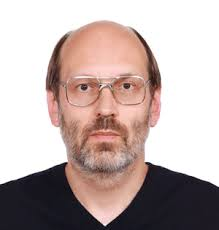
\includegraphics[width=1.2\textwidth]{images/schweizer.jpeg}}
	\caption{\hspace{0.1cm}\scriptsize{Schweizer}}
	\end{subfigure} \\
	%
	\hfill
	\begin{subfigure}{0.12\textwidth}
	\captionsetup{labelformat=empty}
	\centering
	\fbox{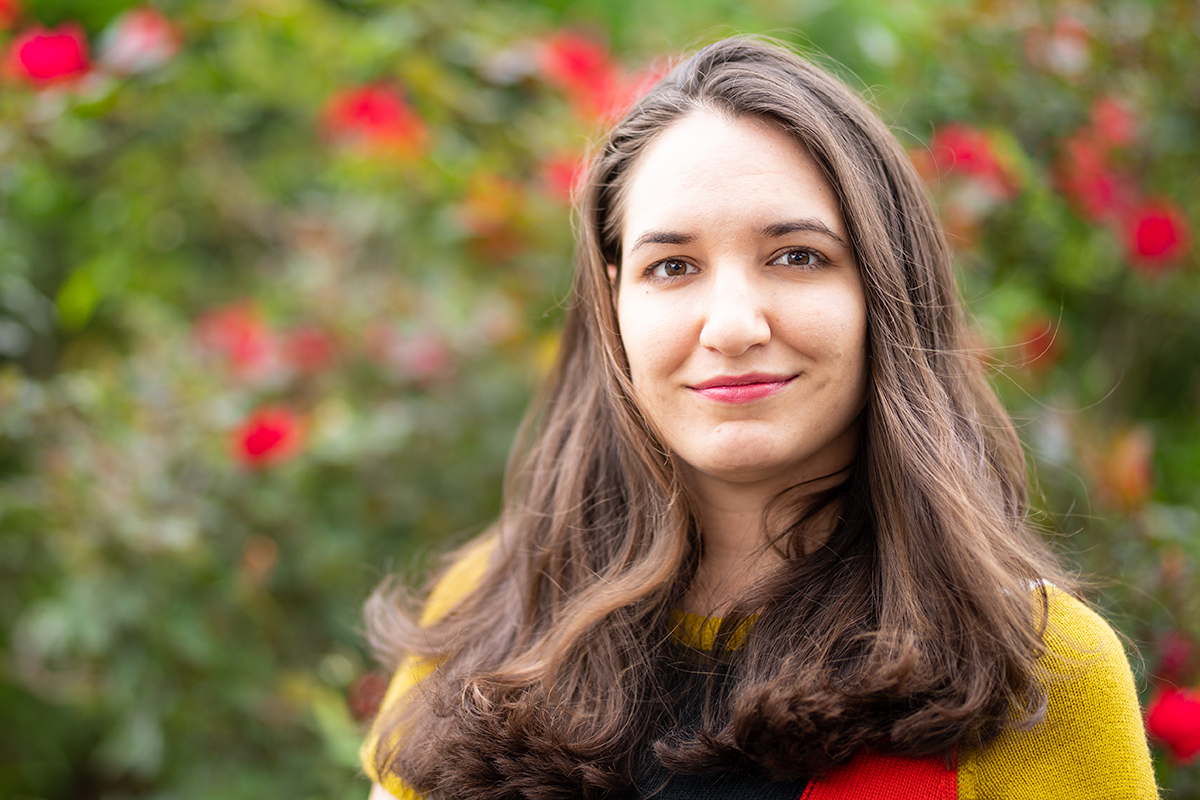
\includegraphics[width=1.5\textwidth]{images/etropolski.jpg}}
	\caption{\;\;\;\;\scriptsize{Etropolski}}
	\end{subfigure} \hfill
	%
	\begin{subfigure}{0.10\textwidth}
	\captionsetup{labelformat=empty}
	\centering
	\fbox{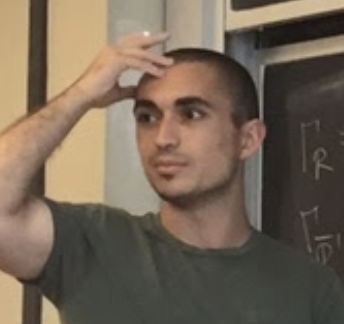
\includegraphics[width=1.5\textwidth]{images/morrow.png}}
	\caption{\;\;\;\scriptsize{Morrow}}
	\end{subfigure} \hfill
	%
	\begin{subfigure}{0.10\textwidth}
	\captionsetup{labelformat=empty}
	\centering
	\fbox{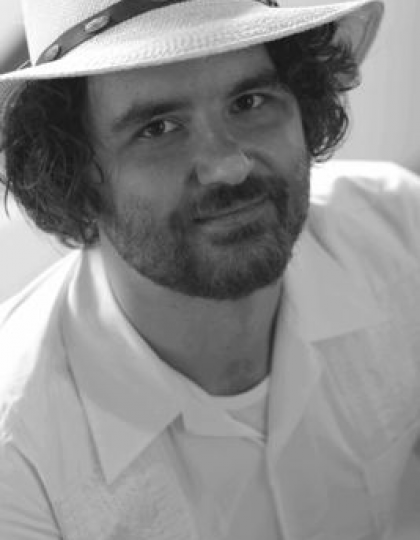
\includegraphics[width=1.2\textwidth]{images/zbrown.png}}
	\caption{\;\;\scriptsize{Z-B.}}
	\end{subfigure} \hfill
	%
	\begin{subfigure}{0.10\textwidth}
	\captionsetup{labelformat=empty}
	\centering
	\fbox{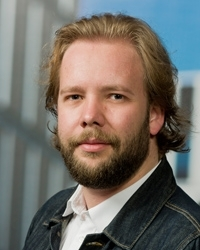
\includegraphics[width=1.2\textwidth]{images/derickx.jpg}}
	\caption{\;\;\scriptsize{Derickx}}
	\end{subfigure} \hfill \phantom{I}
	\end{figure}
\end{frame}



% Quartic
\begin{frame}[plain]
\begin{thm}[Jeon, Kim, Park, 2006]
Let $K/\Q$ be a quartic number field and $E/K$ be an elliptic curve. Then the possible torsion subgroups $E(K)_\tors$ appearing infinitely often are precisely:
	\[
	\begin{cases}
	\Z/n\Z, & n=1,2,\ldots,18,20,21,22 \\
	\Z/2\Z \oplus \Z/2n\Z, & n=1,\ldots,9 \\
	\Z/3\Z \oplus \Z/3n\Z, & n=1,2,3 \\
	\Z/4\Z \oplus \Z/4n\Z, & n=1,2 \\
	\Z/5\Z \oplus \Z/5\Z \\
	\Z/6\Z \oplus \Z/6\Z
	\end{cases}
	\]
\end{thm}
	\begin{figure}[h]
	\centering
	\begin{subfigure}{0.3\textwidth}
	\captionsetup{labelformat=empty}
	\centering
	\fbox{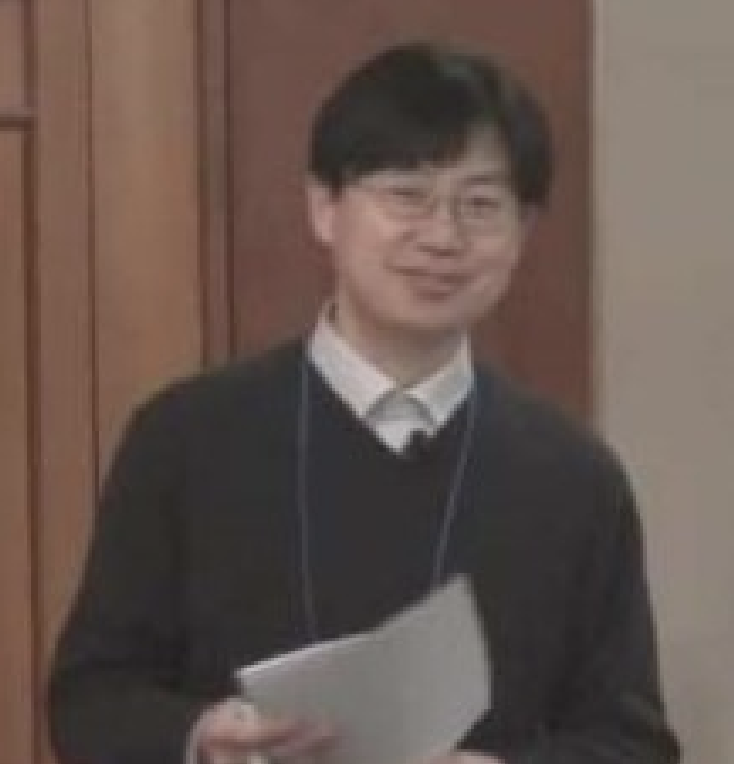
\includegraphics[width=0.60\textwidth]{images/jeon.png}}
	\caption{\hspace{0.1cm}Daeyeol Jeon}
	\end{subfigure}
	%
	\begin{subfigure}{0.3\textwidth}
	\captionsetup{labelformat=empty}
	\centering
	\fbox{
\includegraphics[width=0.63\textwidth]{images/kim.jpg}}
	\caption{Chang Kim}
	\end{subfigure}
	%
	\begin{subfigure}{0.3\textwidth}
	\captionsetup{labelformat=empty}
	\centering
	\fbox{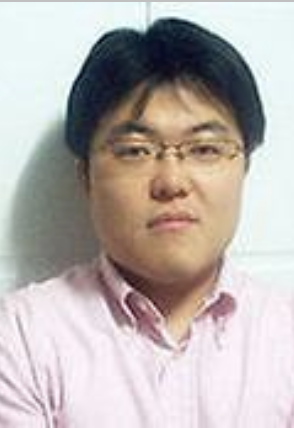
\includegraphics[width=0.45\textwidth]{images/park.png}}
	\caption{\hspace{0cm}Eui-Sung Park}
	\end{subfigure}
	\end{figure}
\end{frame}



% Quintic
\begin{frame}[plain]
\begin{thm}[Derickx, Sutherland, 2016]
Let $K/\Q$ be a quintic number field and $E/K$ be an elliptic curve. Then the possible torsion subgroups $E(K)_\tors$ appearing infinitely often are precisely:
	\[
	\begin{cases}
	\Z/n\Z, & n=1,\ldots,22,24,25 \\
	\Z/2\Z \oplus \Z/2n\Z, & n=1,\ldots,8
	\end{cases}
	\]
\end{thm}
	\begin{figure}[h]
	\centering
	\begin{subfigure}{0.3\textwidth}
	\captionsetup{labelformat=empty}
	\centering
	\fbox{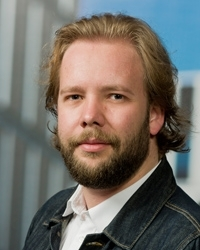
\includegraphics[width=0.72\textwidth]{images/derickx.jpg}}
	\caption{\hspace{0.1cm}Maarten Derickx}
	\end{subfigure}
	%
	\begin{subfigure}{0.3\textwidth}
	\captionsetup{labelformat=empty}
	\centering
	\fbox{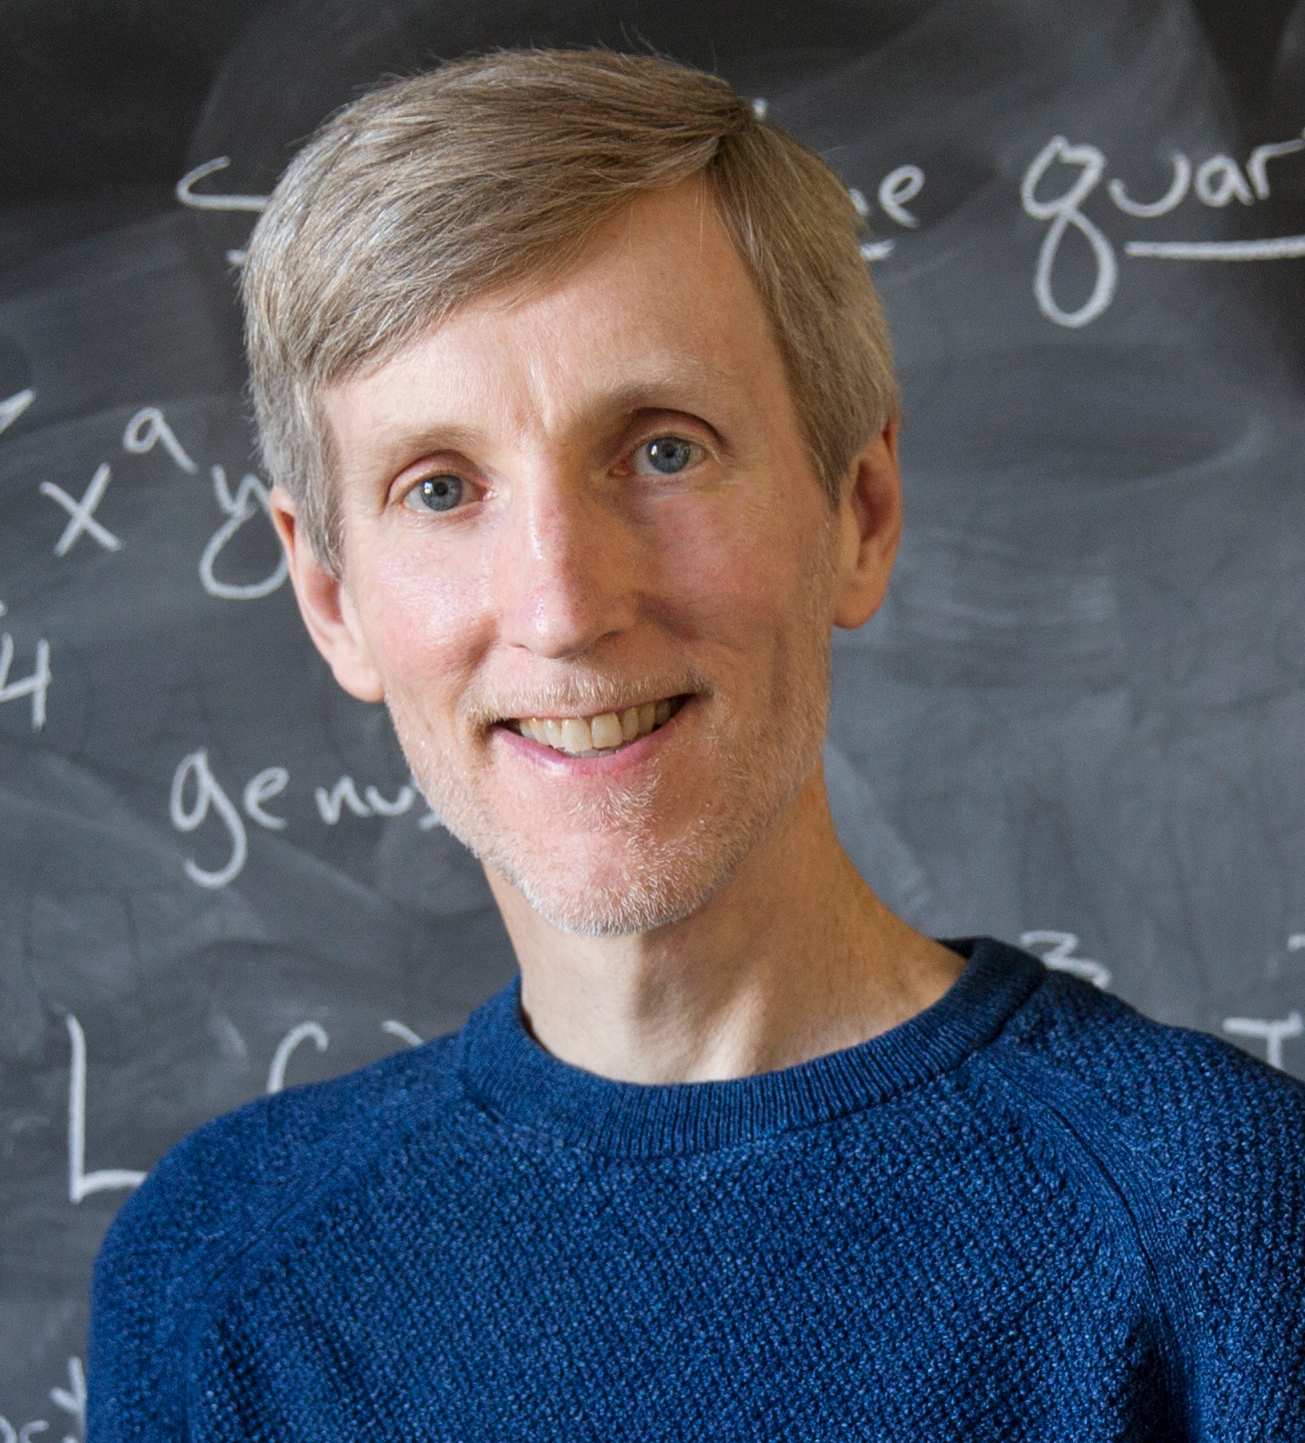
\includegraphics[width=0.82\textwidth]{images/sutherland.jpg}}
	\caption{Drew Sutherland}
	\end{subfigure}
	\end{figure}
\end{frame}



% Sextic
\begin{frame}[plain]
\begin{thm}[Derickx, Sutherland, 2016]
Let $K/\Q$ be a sextic number field and $E/K$ be an elliptic curve. Then the possible torsion subgroups $E(K)_\tors$ appearing infinitely often are precisely:
	\[
	\begin{cases}
	\Z/n\Z, &  n=1,\ldots,30; n \neq 23,25,29 \\
	\Z/2\Z \oplus \Z/2n\Z, & n=1,\ldots,10 \\
	\Z/3\Z \oplus \Z/3n\Z, & n=1,\ldots,4 \\
	\Z/4\Z \oplus \Z/4n\Z, & n=1,2 \\
	\Z/6\Z \oplus \Z/6\Z 
	\end{cases}
	\]
\end{thm}
	\begin{figure}[h]
	\centering
	\begin{subfigure}{0.3\textwidth}
	\captionsetup{labelformat=empty}
	\centering
	\fbox{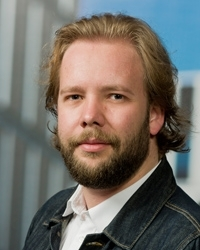
\includegraphics[width=0.72\textwidth]{images/derickx.jpg}}
	\caption{\hspace{0.1cm}Maarten Derickx}
	\end{subfigure}
	%
	\begin{subfigure}{0.3\textwidth}
	\captionsetup{labelformat=empty}
	\centering
	\fbox{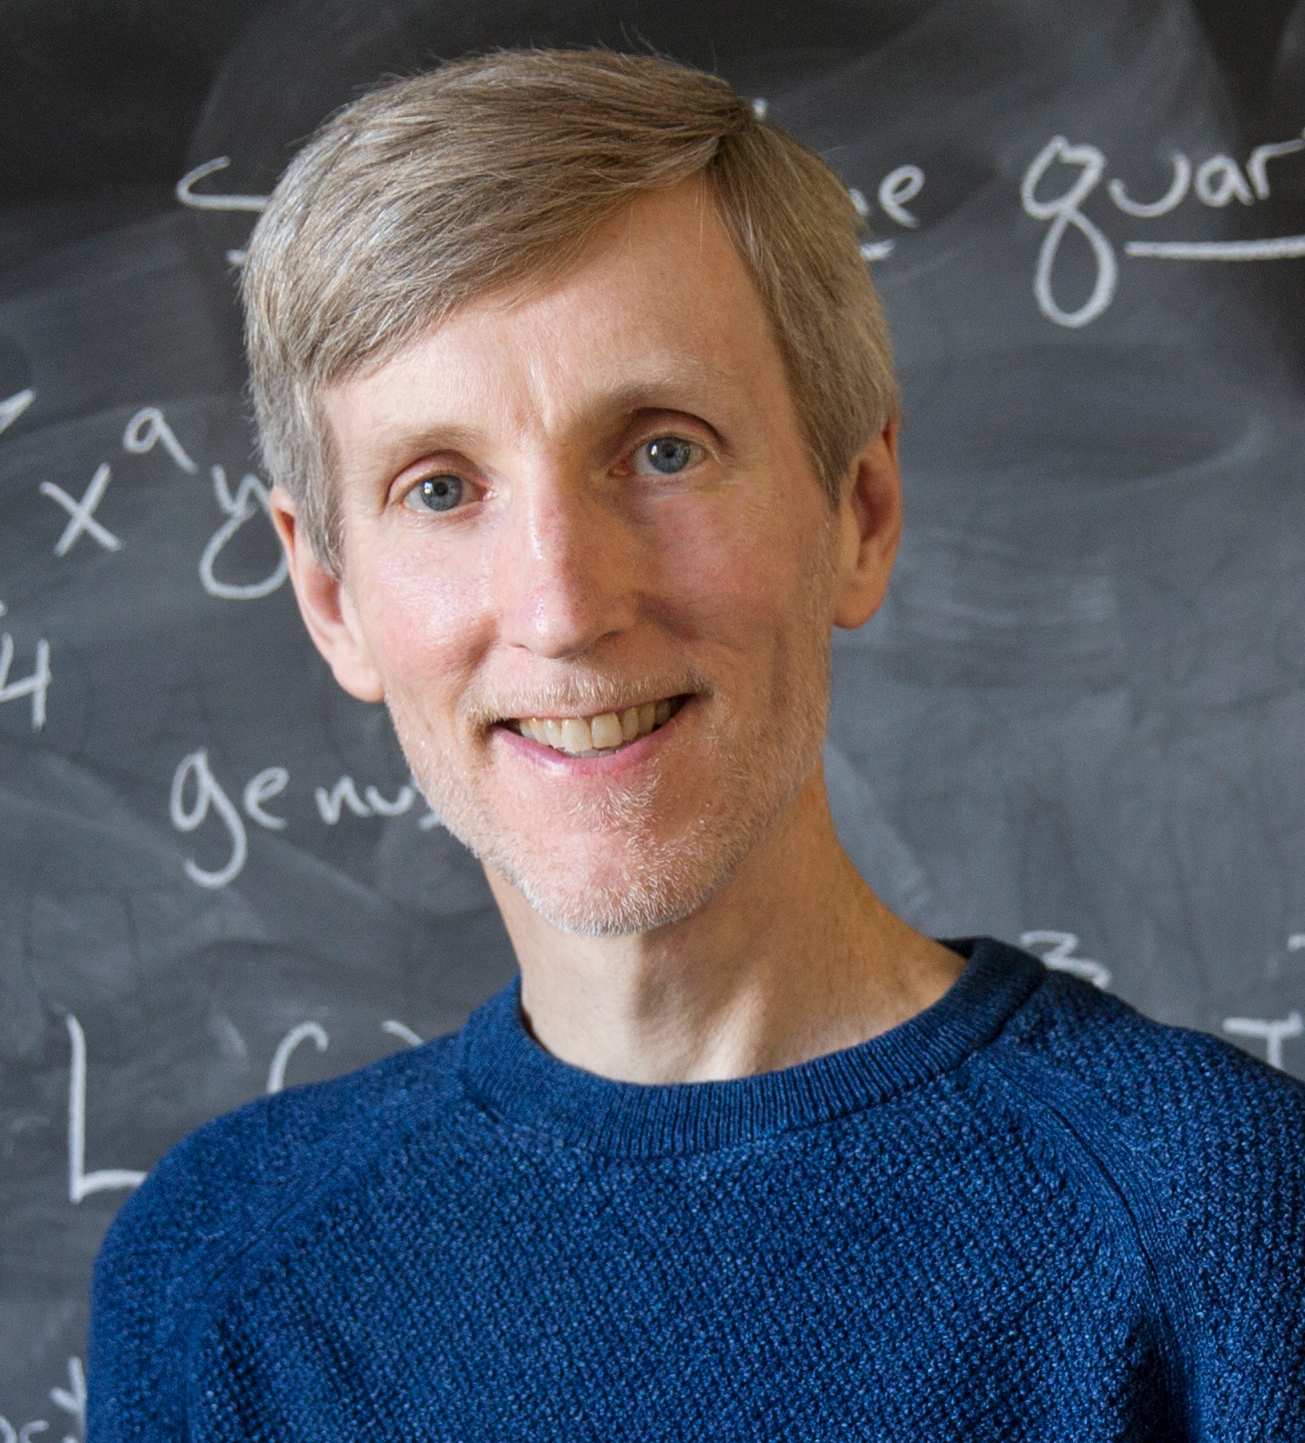
\includegraphics[width=0.82\textwidth]{images/sutherland.jpg}}
	\caption{Drew Sutherland}
	\end{subfigure}
	\end{figure}
\end{frame}



% CM Elliptic Curves
\begin{frame}
\ctext{What about CM Elliptic Curves?}
\end{frame}



% CM 1
\begin{frame}[plain]
	\begin{thm}[Clark, Corn, Rice, Stankewicz; 2013]
	Let $K$ be a number field of degree $d=1,2,\ldots,13$ and $E/K$ be an elliptic curve with CM. Then all possible torsion subgroups are given, and an algorithm to compute the list.
	\end{thm} 
	\begin{figure}[h]
	\centering
	\begin{subfigure}{0.23\textwidth}
	\captionsetup{labelformat=empty}
	\centering
	\fbox{
\includegraphics[width=0.75\textwidth]{images/clark.jpg}}
	\caption{Pete Clark}
	\end{subfigure}
	%
	\begin{subfigure}{0.23\textwidth}
	\captionsetup{labelformat=empty}
	\centering
	\fbox{
\includegraphics[width=0.83\textwidth]{images/corn.jpg}}
	\caption{Patrick Corn}
	\end{subfigure}
	%
	\begin{subfigure}{0.23\textwidth}
	\captionsetup{labelformat=empty}
	\centering
	\fbox{
\includegraphics[width=1.0\textwidth]{images/rice.png}}
	\caption{Alex Rice}
	\end{subfigure}
	%
	\begin{subfigure}{0.25\textwidth}
	\captionsetup{labelformat=empty}
	\centering
	\fbox{
\includegraphics[width=0.65\textwidth]{images/stankewicz.png}}
	\caption{James Stankewicz}
	\end{subfigure}
	\end{figure}
\end{frame}



% CM 2
\begin{frame}[plain]
	\begin{thm}[Bourdon, Pollack; 2018]
	Let $K$ be an odd degree number field and $E/K$ be an elliptic curve with CM. Then the torsion subgroups $E(K)_\tors$ are computable. 
	\end{thm} 
	\begin{figure}[h]
	\centering
	\begin{subfigure}{0.3\textwidth}
	\captionsetup{labelformat=empty}
	\centering
	\fbox{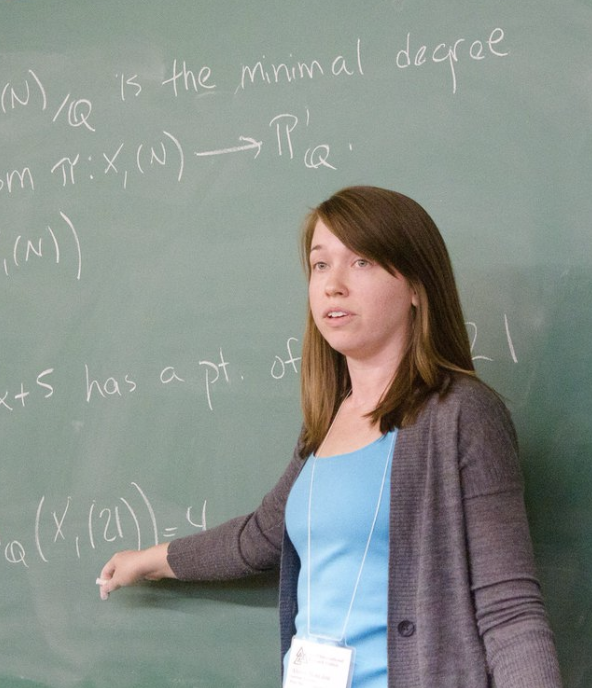
\includegraphics[width=0.85\textwidth]{images/bourdon.png}}
	\caption{Abbey Bourdon}
	\end{subfigure}
	%
	\begin{subfigure}{0.3\textwidth}
	\captionsetup{labelformat=empty}
	\centering
	\fbox{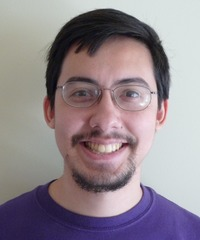
\includegraphics[width=0.82\textwidth]{images/pollack.jpg}}
	\caption{Paul Pollack}
	\end{subfigure}
	\end{figure}
\end{frame}



% Rational EC
\begin{frame}
\ctext{What about Rational Elliptic Curves}
\end{frame}



% Isogeny
\begin{frame}[plain]
	\begin{thm}[Fricke, Kenku, Klein, Kubert, Ligozat, Mazur, Ogg, et al.]
	If $E/\Q$ has an $n$-isogeny over $\Q$, then 
		\[
		n \in \{1,2,\ldots,19,21,25,27,37,43,67,163\}. 
		\]
	If $E$ does not have CM, then $n \leq 18$ or $n \in \{21,25,37\}$. 
	\end{thm}
\end{frame}



% Rational EC
\begin{frame}[plain]
\begin{thm}[Chou,Daniels,Gonz\'alez-Jimenez,Lozano-Robledo,Najman,Tornero,et~al.]
Let $\cC_n$ denote the cyclic subgroup of order $n$. Then 
	\[
	\begin{aligned}
	\Phi_\Q(2)&= \{ \cC_n \colon n= 1,2,\ldots,10,12,15,16\} \\
			&\quad\quad\cup \{ \cC_2 \oplus \cC_{2n} \colon 1,2,\ldots,6\} \cup \{ \cC_3 \oplus \cC_3, \cC_3 \oplus \cC_6, \cC_4 \oplus \cC_4 \} \\
	\Phi_\Q(3)&= \{ \cC_n \colon n=1,2,\ldots,10,12,13,14,18,21 \} \\
			&\quad\quad\cup \{ \cC_2 \oplus \cC_{2n} \colon n=1,2,3,4,7 \} \\
	\Phi_\Q(4)&= \{ \cC_n \colon n=12,\ldots,10,12,13,15,16,20,24 \} \\
			&\quad\quad\cup \{ \cC_2 \oplus \cC_{2n} \colon n=1,2,\ldots,6,8\} \, \cup \{ \cC_3 \oplus \cC_{3n} \colon n=1,2 \} \\
			&\quad\quad\quad\cup \{ \cC_4 \oplus \cC_{4n} \colon n=1,2 \} \cup \{ \cC_5 \oplus \cC_5 \} \cup \{ \cC_6 \oplus \cC_6 \}	\\
	\Phi_\Q(5)&= \{ \cC_n \colon n=1,2,\ldots,12,25\} \cup \{ \cC_2 \oplus \cC_{2n} \colon n=1,2,3,4\} \\
	\Phi_\Q(6)&\supseteq \{ \cC_n \colon n=1,2,\ldots,21,30 \colon n \neq 11,17,19,20\} \\
			&\quad\quad\cup \{ \cC_2 \oplus \cC_{2n} \colon n=1,2,\ldots,7,9 \} \\
			&\quad\quad\quad\cup \{ \cC_3 \oplus \cC_{3n} \colon n=1,2,3,4\} \cup \{ \cC_4 \oplus \cC_4, \cC_6 \oplus \cC_6 \} \\
	\Phi_\Q(d^*)&= \Phi_\Q(1)
	\end{aligned}
	\]
\end{thm}
\end{frame}



% Photos
\begin{frame}[plain]
	\begin{figure}[h]
	\centering
	\begin{subfigure}{0.25\textwidth}
	\captionsetup{labelformat=empty}
	\centering
	\fbox{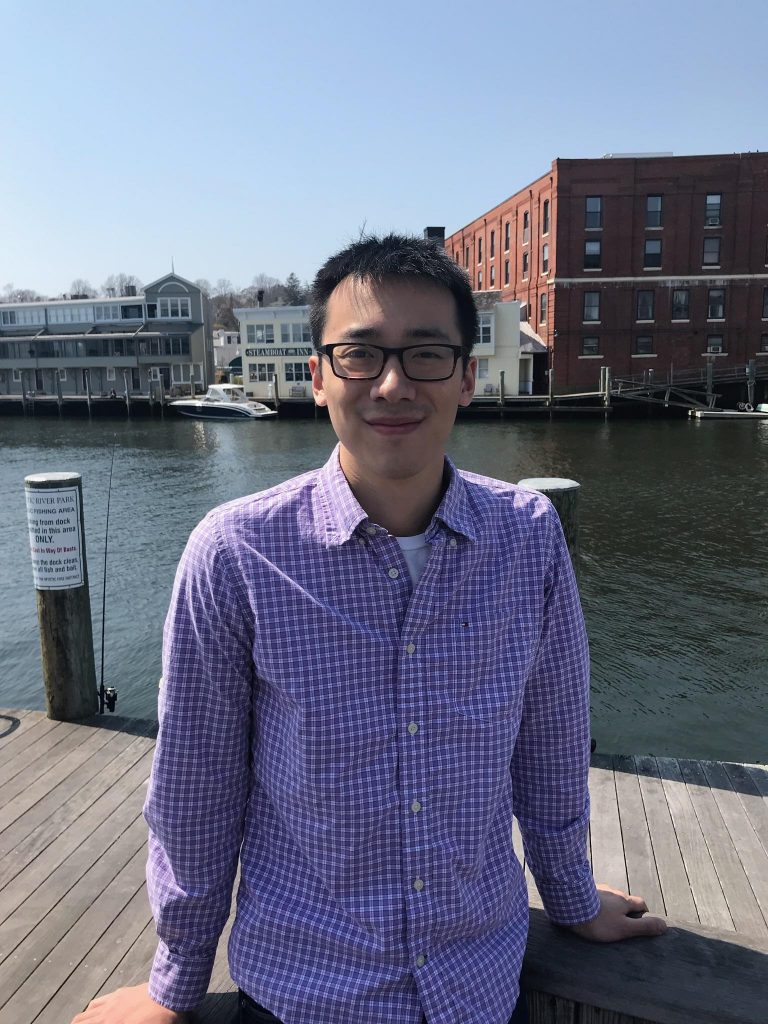
\includegraphics[width=0.70\textwidth]{images/chou.jpg}}
	\caption{Michael Chou}
	\end{subfigure} \quad\quad
	%
	\begin{subfigure}{0.25\textwidth}
	\captionsetup{labelformat=empty}
	\centering
	\fbox{
\includegraphics[width=0.90\textwidth]{images/daniels.jpeg}}
	\caption{Harris Daniels}
	\end{subfigure} \enskip
	%
	\begin{subfigure}{0.35\textwidth}
	\captionsetup{labelformat=empty}
	\centering
	\fbox{
\includegraphics[width=0.50\textwidth]{images/jimenez.png}}
	\caption{Enrique Gonz\'alez-Jim\'enez}
	\end{subfigure} \\
	%
	\begin{subfigure}{0.35\textwidth}
	\captionsetup{labelformat=empty}
	\centering
	\fbox{
\includegraphics[width=0.6\textwidth]{images/robledo.jpg}}
	\caption{\'Alvaro Lozano-Robledo}
	\end{subfigure} \quad
	%
	\begin{subfigure}{0.25\textwidth}
	\captionsetup{labelformat=empty}
	\centering
	\fbox{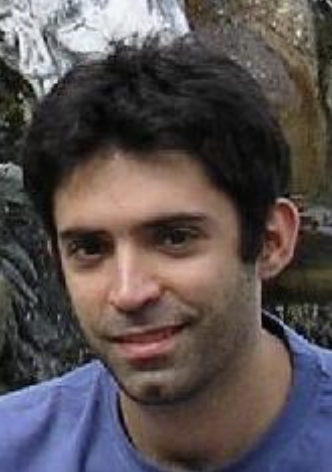
\includegraphics[width=0.62\textwidth]{images/najman2.png}}
	\caption{Filip Najman}
	\end{subfigure} \quad\quad
	%
	\begin{subfigure}{0.25\textwidth}
	\captionsetup{labelformat=empty}
	\centering
	\fbox{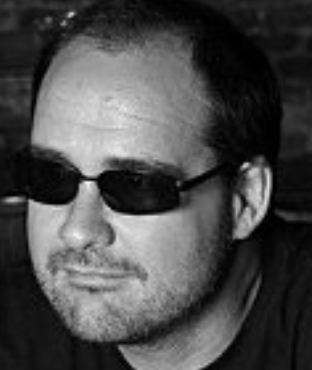
\includegraphics[width=0.75\textwidth]{images/tornero.png}}
	\caption{Jos\'e Tornero}
	\end{subfigure}
	\end{figure}
\end{frame}



% The Results
\begin{frame}[plain]
\vfill
\begin{center} {\bfseries \Large \textcolor{UniGray}{The Result for Nonic Galois Fields}} \end{center}
\vfill 
\end{frame}



% Result
\begin{frame}[plain]
\begin{thm}[M.]
Let $K/\Q$ be a nonic Galois field, and let $E/\Q$ be a rational elliptic curve. Then the possible torsion subgroups $E(K)_\tors$ are precisely:
	\[
	\begin{cases}
	\Z/n\Z, & n=1,2,\ldots,10,12,13,14,18,19,21,27 \\
	\Z/2\Z \oplus \Z/2n\Z, & n=1,2,3,4,7
	\end{cases}
	\]
\end{thm}
\end{frame}



% Result 2
\begin{frame}[plain]
\begin{thm}[M.]
Let $K/\Q$ be a nonic Galois field with $\Gal(K/\Q) \cong \Z/3\Z \oplus \Z/3\Z$, and let $E/\Q$ be a rational elliptic curve. Then the possible torsion subgroups $E(K)_\tors$ are precisely:
	\[
	\begin{cases}
	\Z/n\Z, & n=1,2,\ldots,10,12,13,14,18,21 \\
	\Z/2\Z \oplus \Z/2n\Z, & n=1,2,3,4,7
	\end{cases}
	\]
\end{thm}
\end{frame}



% Result 3
\begin{frame}[plain]
\begin{thm}[M.]
Let $K/\Q$ be a nonic Galois field with $\Gal(K/\Q) \cong \Z/9\Z$, and let $E/\Q$ be a rational elliptic curve. Then the possible torsion subgroups $E(K)_\tors$ are:
	\[
	\begin{cases}
	\Z/n\Z, & n=1,2,\ldots,10,12,13^*,18^*,19,21,27 \\
	\Z/2\Z \oplus \Z/2n\Z, & n=1,2,3,4
	\end{cases}
	\]
\end{thm}
\end{frame}



% Outline
\begin{frame}[plain]
\vfill
\begin{center} {\bfseries \Large \textcolor{UniGray}{Outline of the Method}} \end{center}
\vfill 
\end{frame}



% Step 1
\begin{frame}[plain]
\vfill
\begin{center} {\bfseries \Large \textcolor{UniGray}{Step 1. Determine the Possible Prime Orders}} \end{center}
\vfill 
\end{frame}



% Primes 1
\begin{frame}[plain]
\begin{thm}[Lozano-Robledo]
Let $S_\Q(d)$ be the set of primes such that there exists an elliptic curve $E/\Q$ with a point of order $p$ defined in an extension $K/\Q$ of degree at most $d$. Then $S_\Q(9)= \{2,3,5,7,11,13,17,19\}$.
\end{thm}
	\begin{figure}[h]
	\centering
	\begin{subfigure}{\textwidth}
	\captionsetup{labelformat=empty}
	\centering
	\fbox{
\includegraphics[width=0.2\textwidth]{images/robledo.jpg}}
	\caption{\'Alvaro Lozano-Robledo}
	\end{subfigure}
	\end{figure}
\begin{rem}
Lozano-Robledo computes $S_\Q(d)$ for $1 \leq d \leq 21$, and gives a conjecturally formula valid for all $1 \leq d \leq 42$, following from a positive answer to Serre's uniformity question.
\end{rem}
\end{frame}



% Primes 2
\begin{frame}[plain]
\begin{prop}[Gonz\'alez-Jim\'enez, Najman] \hfill
	\begin{enumerate}[(i)]
	\item $11 \in R_\Q(d)$ if and only if $5 \mid d$.
	\item $13 \in R_\Q(d)$ if and only if $3 \mid d$ or $4 \mid d$. 
	\item $17 \in R_\Q(d)$ if and only if $8 \mid d$.
	\end{enumerate}
\end{prop}
	\begin{figure}[h]
	\centering
	\begin{subfigure}{0.35\textwidth}
	\captionsetup{labelformat=empty}
	\centering
	\fbox{
\includegraphics[width=0.65\textwidth]{images/jimenez.png}}
	\caption{Enrique Gonz\'alez-Jim\'enez}
	\end{subfigure}
	%
	\begin{subfigure}{0.3\textwidth}
	\captionsetup{labelformat=empty}
	\centering
	\fbox{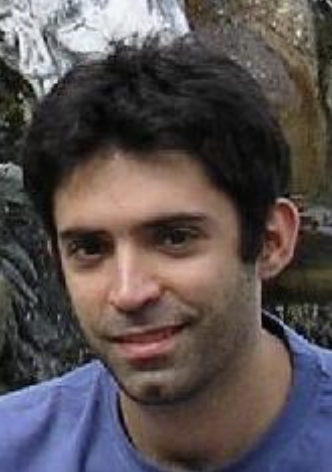
\includegraphics[width=0.70\textwidth]{images/najman2.png}}
	\caption{Filip Najman}
	\end{subfigure}
	\end{figure}
\end{frame}



% Prime Possible
\begin{frame}[plain]
\begin{prop}
Let $E/\Q$ be a rational elliptic curve, and let $K/\Q$ be a nonic Galois field. Then if $P \in E(K)$ is a point of prime order $p$, then $p \in \{2,3,5,7,13,19\}$.
\end{prop}
\end{frame}



% Step 2
\begin{frame}[plain]
\vfill
\begin{center} {\bfseries \Large \textcolor{UniGray}{Step 2. Bound the Size of the Sylow Subgroups}} \end{center}
\vfill 
\end{frame}



% Weil
\begin{frame}[plain]
\begin{lem}
Let $K/\Q$ be an odd degree number field, and let $E/\Q$ be a rational elliptic curve. Then $E(K)_\tors$ does not contain full $p$-torsion for all odd primes.
\end{lem}
\end{frame}



% Isogeny
\begin{frame}[plain]
\begin{lem}
Let $K/\Q$ be a Galois extension, and let $E/\Q$ be a rational elliptic curve. If $E(K)[n] \cong \Z/n\Z$, then $E$ has a rational $n$-isogeny. 
\end{lem}
\end{frame}



% Isogeny
\begin{frame}[plain]
	\begin{thm}[Fricke, Kenku, Klein, Kubert, Ligozat, Mazur, Ogg, et al.]
	If $E/\Q$ has an $n$-isogeny over $\Q$, then 
		\[
		n \in \{1,2,\ldots,19,21,25,27,37,43,67,163\}. 
		\]
	If $E$ does not have CM, then $n \leq 18$ or $n \in \{21,25,37\}$. 
	\end{thm}
\end{frame}



% Sylow Bound
\begin{frame}[plain]
\begin{lem}
Let $E/\Q$ be a rational elliptic curve, and let $K/\Q$ be a nonic Galois field. Then
	\[
	\begin{aligned}
	E(K)[3^\infty]&\subseteq \Z/27\Z \\
	E(K)[5^\infty]&\subseteq \Z/25\Z \\
	E(K)[7^\infty]&\subseteq \Z/7\Z \\
	E(K)[13^\infty]&\subseteq \Z/13\Z \\
	E(K)[19^\infty]&\subseteq \Z/19\Z
	\end{aligned}
	\]
\end{lem}
\end{frame}



% 2-adic
\begin{frame}[plain]
\begin{thm}[Rouse,Zureick-Brown, 2015]
Let $E/\Q$ be a rational elliptic curve without CM. Then the index of $\rho_{E,2^\infty}(\Gal(\overline{\Q}/\Q))$ divides 64 or 96, and all such indices occur. Furthermore, the image of $\rho_{E,2^\infty}(\Gal(\overline{\Q}/\Q))$ is the inverse image in $\GL_2(\Z_2)$ of the image of $\rho_{E,32}(\Gal(\overline{\Q}/\Q))$.
\end{thm}
	\begin{figure}[h]
	\centering
	\begin{subfigure}{0.3\textwidth}
	\captionsetup{labelformat=empty}
	\centering
	\fbox{\includegraphics[width=0.70\textwidth]{images/rouse.jpg}}
	\caption{Jeremy Rouse}
	\end{subfigure}
	%
	\begin{subfigure}{0.3\textwidth}
	\captionsetup{labelformat=empty}
	\centering
	\fbox{\includegraphics[width=0.69\textwidth]{images/zbrown.png}}
	\caption{David Zureick-Brown}
	\end{subfigure}
	\end{figure}
\begin{rem}
They also enumerate all 1,208 possibilities and find their rational points. 
\end{rem}
\end{frame}



% Full 2-torsion
\begin{frame}[plain]
\begin{thm}[Gonz\'alez-Jim\'enez, Lozano-Robledo]
Let $E/\Q$ be an elliptic curve without CM. Let $1 \leq s \leq N$ be fixed integers, and let $T \subseteq E[2^N]$ be a subgroup isomorphic to $\Z/2^s/Z \oplus \Z/2^N \Z$. Then $[\Q(T) \colon \Q]$ is divisible by 2 if $s=N=2$, and otherwise by $2^{2N+2s-8}$ if $N \geq 3$, unless $s \geq 4$ and $j(E)$ is one of the two values:
	\[
	- \dfrac{3 \cdot 18249920^3}{17^{16}}\; \text{ or } - \dfrac{7 \cdot 1723187806080^3}{79^{16}}
	\]
in which case $[\Q(T) \colon \Q]$ is divisible by $3 \cdot 2^{2N+2s-9}$. Moreover, this is best possible in that there are one-parameter families $E_{s,N}(t)$ of elliptic curves over $\Q$ such that for each $s, N \geq 0$ and each $t \in \Q$, and subgroups $T_{s,N} \in E_{s,N}(t)(\ov{\Q})$ isomorphic to $\Z/2^s\Z \oplus \Z/2^N\Z$ such that $[\Q(T_{s,N}) \colon \Q]$ is equal to the bound given above. 
\end{thm}
\end{frame}



% Sylow Bound
\begin{frame}[plain]
\begin{lem}
Let $E/\Q$ be a rational elliptic curve, and let $K/\Q$ be a nonic Galois field. Then $E(K)[2^\infty] \subseteq \Z/2\Z \oplus \Z/16\Z$.
\end{lem}
\end{frame}



% Combined
\begin{frame}[plain]
\begin{prop}
Let $E/\Q$ be a rational elliptic curve, and let $K/\Q$ be a nonic Galois field. Then \par\vspace{\baselineskip}

\small{$E(K)_\tors \subseteq (\Z/2\Z \oplus \Z/16\Z) \oplus \Z/27\Z \oplus \Z/25\Z \oplus \Z/7\Z \oplus \Z/13\Z \oplus \Z/19\Z$}. \par\vspace{\baselineskip}
\end{prop}
\end{frame}



% Step 3
\begin{frame}[plain]
\vfill
\begin{center} {\bfseries \Large \textcolor{UniGray}{Step 3. Eliminate Possibilities}} \end{center}
\vfill 
\end{frame}


%
%
%
%
%
%
% More Here?
%
%
%
%
%



% Fields of Def.
\begin{frame}[plain]
\begin{lem}
Let $K/\Q$ be a nonic Galois field, and let $E/\Q$ be a rational elliptic curve. Let $P \in E(K)$ be a point of order $p$. 
	\begin{enumerate}
	\item If $p= 2,3,5$, then $P$ is rational or defined over a cubic field.
	\item If $p= 7, 13, 19$, then $P$ is defined over a cubic field.
	\end{enumerate}
\end{lem}
\end{frame}



% Galois 1
\begin{frame}[plain]
\begin{lem}[Najman]
Let $p, q$ be distinct odd primes, $F_2/F_1$ a Galois extension of number fields such that $\Gal(F_2/F_1) \simeq \Z/q\Z$ and $E/F_1$ an elliptic curve with no $p$-torsion over $F_1$. Then if $q$ does not divide $p-1$ and $\Q(\zeta_p) \not\subset F_2$, then $E(F_2)[p]=0$. 
\end{lem}

\begin{lem}[Najman]
Let $p$ be an odd prime number, $q$ a prime not dividing $p$, $F_2/F_1$ a Galois extension of number fields such that $\Gal(F_2/F_1) \simeq \Z/q\Z$, $E/F_1$ an elliptic curve, and suppose $E(F_1) \supset \Z/p\Z$, $E(F_1) \not\supset \Z/p^2\Z$, and $\zeta_p \notin F_2$. Then $E(F_2) \not\supset \Z/p^2\Z$.
\end{lem}
\end{frame}



% 2-Sylow, 5-Sylow
\begin{frame}[plain]
\begin{prop}[Najman]
Let $K$ be a cubic field. Then the 5-Sylow groups of $E(\Q)$ and $E(K)$ are equal. 
\end{prop} \pause

\begin{prop}[Najman]
If the torsion subgroup of an elliptic curve $E$ over $\Q$ has a nontrivial 2-Sylow subgroup, then over any number field of odd degree the torsion of $E$ will have the same 2-Sylow subgroup as over $\Q$.
\end{prop} \pause

\begin{prop}
Let $E/\Q$ be a rational elliptic curve, and let $K/\Q$ be a nonic Galois field. Let $F$ be cubic subfield of $K$. If the 2-Sylow subgroup of $E(F)_\tors$ is nontrivial, then $E(K)[2^\infty]=E(F)[2^\infty]$.
\end{prop}

\end{frame}



% 5-Sylow
\begin{frame}[plain]
\begin{prop}
Let $E/\Q$ be a rational elliptic curve, and let $K/\Q$ be a nonic Galois field. Then $E(K)_\tors$ does not contain $\Z/2\Z \oplus \Z/10\Z$.
\end{prop} \pause

\begin{prop}
Let $E/\Q$ be a rational elliptic curve, and let $K/\Q$ be a nonic Galois field. Then $E(K)_\tors$ does not contain $\Z/15\Z$.
\end{prop}
\end{frame}



% Z/16Z
\begin{frame}[plain]
\begin{prop}
Let $E/\Q$ be a rational elliptic curve, and let $K/\Q$ be a nonic Galois field. Then $E(K)_\tors$ does not contain $\Z/16\Z$.
\end{prop} \pause

\pf 
\begin{itemize}
\item We know $\Z/2\Z \oplus \Z/16\Z$ is not an option. \pause
\item If $E(\Q)[2^\infty] \neq \{\O\}$, then $E(\Q)[2^\infty] \supseteq \Z/16\Z$. 
\item $E(K)[16] \cong \Z/16\Z$ so $E$ has a 16-isogeny. \pause
\item Choose a model $E: y^2= x^3+Ax+B$. 
\item Then $\Q(x^3+Ax+B) \subseteq K$ is a cubic field. \pause
\item We must have $\disc f(x)= \square$. \pause
\item $j= \dfrac{(h^8-16h^4+16)^3}{h^4(h^4-16)}$ for $h \in \Q \setminus \{0,\pm2\}$.
\end{itemize}
\end{frame}



% Cont
\begin{frame}[plain]
For $h \in \Q \setminus \{0,\pm2\}$, $E$ must be
	\[
	y^2= x^3 - \dfrac{27(h^8-16h^4+16)^3}{(h^{12}-24h^8+120h^4+64)^2} \,x + \dfrac{54(h^8-16h^4+16)^3}{(h^{12}-24h^8+120h^4+64)^2}
	\] \pause
Its discriminant must be a square, so
	\[
	M^2= \dfrac{136048896h^4(h^4-16)(h^8-16h^4+16)^6}{(h^{12}-24h^8+120h^4+64)^6}
	\] \pause
Any solution is a subset of the rational points on the curve
	\[
	X: y^2= h^4 - 16
	\] \pause
$X(\Q)= \{\O,(8,24),(0,8),(-4,0),(0,-8),(8,-24)\}$, none of which are solutions.
\end{frame}



% Bicyclic
\begin{frame}[plain]
\vfill
\begin{center} {\bfseries \Large \textcolor{UniGray}{Nonic Bicyclic Galois Fields}} \end{center}
\vfill 
\end{frame}



% Cubic Compositum
\begin{frame}[plain]
\begin{thm}[Daniels, Lozano-Robledo, Najman, Sutherland, 2017]
Let $E/\Q$ be a rational elliptic curve. Then $E(\Q(3^\infty))_\tors$ is finite and is isomorphic to one of the following:
	\[
	\begin{cases}
	\Z/2\Z \oplus \Z/2n\Z, & n=1,2,4,5,7,8,13 \\
	\Z/4\Z \oplus \Z4n\Z, & n=1,2,4,7 \\
	\Z/6\Z \oplus \Z/6n\Z, &  n=1,2,3,5,7 \\
	\Z/2n\Z \oplus \Z/2n\Z, & n=4,6,7,9
	\end{cases}
	\]
\end{thm}
	\begin{figure}[h]
	\centering
	\begin{subfigure}{0.20\textwidth}
	\captionsetup{labelformat=empty}
	\centering
	\fbox{\includegraphics[width=1.05\textwidth]{images/daniels.jpeg}}
	\caption{{\scriptsize Harris Daniels}}
	\end{subfigure}
	%
	\begin{subfigure}{0.325\textwidth}
	\captionsetup{labelformat=empty}
	\centering
	\fbox{\includegraphics[width=0.65\textwidth]{images/robledo.jpg}}
	\caption{{\scriptsize \'Alvaro Lozano-Robledo}}
	\end{subfigure}
	%
	\begin{subfigure}{0.20\textwidth}
	\captionsetup{labelformat=empty}
	\centering
	\fbox{\includegraphics[width=0.75\textwidth]{images/najman2.png}}
	\caption{{\scriptsize Filip Najman}}
	\end{subfigure}
	%
	\begin{subfigure}{0.20\textwidth}
	\captionsetup{labelformat=empty}
	\centering
	\fbox{\includegraphics[width=0.98\textwidth]{images/sutherland.jpg}}
	\caption{{\scriptsize Drew Sutherland}}
	\end{subfigure}
	\end{figure}
\end{frame}



% Najman Cubic
\begin{frame}[plain]
\begin{thm}[Najman]
Let $K/\Q$ be a cubic number field, and let $E/\Q$ be a rational elliptic curve. Then
	\[
	E(F)_\tors \cong
	\begin{cases}
	\Z/n\Z, & n=1,\ldots,10,12,13,14,18,21 \\
	\Z/2\Z \oplus \Z/2n\Z, & n=1,\ldots,4,7
	\end{cases}
	\]
Moreover, the elliptic curve 162B1 over $\Q(\zeta_9)^+$ is the unique rational elliptic curve over a cubic number field with torsion subgroup $\Z/21\Z$.
\end{thm}
	\begin{figure}
	\captionsetup{labelformat=empty}
	\centering
	\fbox{\includegraphics[width=0.30\textwidth]{images/najman.jpg}}
	\caption{\hspace{0.1cm}Filip Najman}
	\end{figure}
\end{frame}



% Cyclic
\begin{frame}[plain]
\vfill
\begin{center} {\bfseries \Large \textcolor{UniGray}{Nonic Cyclic Galois Fields}} \end{center}
\vfill 
\end{frame}



% Cyclic
\begin{frame}[plain]
\begin{prop}
Let $K/\Q$ be a nonic Galois field with $\Gal(K/\Q) \cong \Z/9\Z$, and let $E/\Q$ be a rational elliptic curve. Then $E(K)_\tors$ does not contain a subgroup isomorphic to $\Z/14\Z$.
\end{prop} \pause

\pfsk
\begin{itemize}
\item Assume $K/F/\Q$ exists. Then $E(K)$ has a 14-isogeny. \pause
\item Then $E$ has $j$-invariant $j= -3^3 \cdot 5^3$ or $3^3 \cdot 5^3 \cdot 17^3$, so $E$ must be the latter. \pause
\item Using division polynomials, it must be that $F= \Q(\zeta_7)^+$. \pause
\item $F \subseteq K \subseteq \Q(\zeta_N)$ for some $N= 7^sm$. \pause
\item $|(\Z/7^s\Z)^\times|= 7^{s-1} (7-1)= 6 \cdot 7^{s-1}= 2 \cdot 3 \cdot 7^{s-1}$  \pause
\item CRT produces $u \in \N$ with $\zeta_N \mapsto \zeta_N^u$ automorphism of $K$ of order 3 \pause
\item $\zeta_N \mapsto \zeta_N^u$ non-trivial in $F, K$, contradiction
\end{itemize}
\qed 
\end{frame}



% Questions
\begingroup
\setbeamercolor{background canvas}{bg= gray, fg=white}
\begin{frame}[plain]
\phantom{x} \vfill
\begin{center} {\huge \textcolor{white}{Questions?}} \end{center}
\vfill
\end{frame}
\endgroup